% Options for packages loaded elsewhere
% Options for packages loaded elsewhere
\PassOptionsToPackage{unicode}{hyperref}
\PassOptionsToPackage{hyphens}{url}
\PassOptionsToPackage{dvipsnames,svgnames,x11names}{xcolor}
%
\documentclass[
  number,
  preprint,
  3p,
  onecolumn]{elsarticle}
\usepackage{xcolor}
\usepackage{amsmath,amssymb}
\setcounter{secnumdepth}{5}
\usepackage{iftex}
\ifPDFTeX
  \usepackage[T1]{fontenc}
  \usepackage[utf8]{inputenc}
  \usepackage{textcomp} % provide euro and other symbols
\else % if luatex or xetex
  \usepackage{unicode-math} % this also loads fontspec
  \defaultfontfeatures{Scale=MatchLowercase}
  \defaultfontfeatures[\rmfamily]{Ligatures=TeX,Scale=1}
\fi
\usepackage{lmodern}
\ifPDFTeX\else
  % xetex/luatex font selection
\fi
% Use upquote if available, for straight quotes in verbatim environments
\IfFileExists{upquote.sty}{\usepackage{upquote}}{}
\IfFileExists{microtype.sty}{% use microtype if available
  \usepackage[]{microtype}
  \UseMicrotypeSet[protrusion]{basicmath} % disable protrusion for tt fonts
}{}
\makeatletter
\@ifundefined{KOMAClassName}{% if non-KOMA class
  \IfFileExists{parskip.sty}{%
    \usepackage{parskip}
  }{% else
    \setlength{\parindent}{0pt}
    \setlength{\parskip}{6pt plus 2pt minus 1pt}}
}{% if KOMA class
  \KOMAoptions{parskip=half}}
\makeatother
% Make \paragraph and \subparagraph free-standing
\makeatletter
\ifx\paragraph\undefined\else
  \let\oldparagraph\paragraph
  \renewcommand{\paragraph}{
    \@ifstar
      \xxxParagraphStar
      \xxxParagraphNoStar
  }
  \newcommand{\xxxParagraphStar}[1]{\oldparagraph*{#1}\mbox{}}
  \newcommand{\xxxParagraphNoStar}[1]{\oldparagraph{#1}\mbox{}}
\fi
\ifx\subparagraph\undefined\else
  \let\oldsubparagraph\subparagraph
  \renewcommand{\subparagraph}{
    \@ifstar
      \xxxSubParagraphStar
      \xxxSubParagraphNoStar
  }
  \newcommand{\xxxSubParagraphStar}[1]{\oldsubparagraph*{#1}\mbox{}}
  \newcommand{\xxxSubParagraphNoStar}[1]{\oldsubparagraph{#1}\mbox{}}
\fi
\makeatother


\usepackage{longtable,booktabs,array}
\usepackage{calc} % for calculating minipage widths
% Correct order of tables after \paragraph or \subparagraph
\usepackage{etoolbox}
\makeatletter
\patchcmd\longtable{\par}{\if@noskipsec\mbox{}\fi\par}{}{}
\makeatother
% Allow footnotes in longtable head/foot
\IfFileExists{footnotehyper.sty}{\usepackage{footnotehyper}}{\usepackage{footnote}}
\makesavenoteenv{longtable}
\usepackage{graphicx}
\makeatletter
\newsavebox\pandoc@box
\newcommand*\pandocbounded[1]{% scales image to fit in text height/width
  \sbox\pandoc@box{#1}%
  \Gscale@div\@tempa{\textheight}{\dimexpr\ht\pandoc@box+\dp\pandoc@box\relax}%
  \Gscale@div\@tempb{\linewidth}{\wd\pandoc@box}%
  \ifdim\@tempb\p@<\@tempa\p@\let\@tempa\@tempb\fi% select the smaller of both
  \ifdim\@tempa\p@<\p@\scalebox{\@tempa}{\usebox\pandoc@box}%
  \else\usebox{\pandoc@box}%
  \fi%
}
% Set default figure placement to htbp
\def\fps@figure{htbp}
\makeatother





\setlength{\emergencystretch}{3em} % prevent overfull lines

\providecommand{\tightlist}{%
  \setlength{\itemsep}{0pt}\setlength{\parskip}{0pt}}



 
\usepackage[]{natbib}
\bibliographystyle{elsarticle-num}


\usepackage{booktabs}
\usepackage{longtable}
\usepackage{array}
\usepackage{multirow}
\usepackage{wrapfig}
\usepackage{float}
\usepackage{colortbl}
\usepackage{pdflscape}
\usepackage{tabu}
\usepackage{threeparttable}
\usepackage{threeparttablex}
\usepackage[normalem]{ulem}
\usepackage{makecell}
\usepackage{xcolor}
\usepackage{caption}
\usepackage{anyfontsize}
\usepackage{dcolumn}
\usepackage{typearea}
\usepackage{longtable}
\makeatletter
\@ifpackageloaded{caption}{}{\usepackage{caption}}
\AtBeginDocument{%
\ifdefined\contentsname
  \renewcommand*\contentsname{Table of contents}
\else
  \newcommand\contentsname{Table of contents}
\fi
\ifdefined\listfigurename
  \renewcommand*\listfigurename{List of Figures}
\else
  \newcommand\listfigurename{List of Figures}
\fi
\ifdefined\listtablename
  \renewcommand*\listtablename{List of Tables}
\else
  \newcommand\listtablename{List of Tables}
\fi
\ifdefined\figurename
  \renewcommand*\figurename{Figure}
\else
  \newcommand\figurename{Figure}
\fi
\ifdefined\tablename
  \renewcommand*\tablename{Table}
\else
  \newcommand\tablename{Table}
\fi
}
\@ifpackageloaded{float}{}{\usepackage{float}}
\floatstyle{ruled}
\@ifundefined{c@chapter}{\newfloat{codelisting}{h}{lop}}{\newfloat{codelisting}{h}{lop}[chapter]}
\floatname{codelisting}{Listing}
\newcommand*\listoflistings{\listof{codelisting}{List of Listings}}
\makeatother
\makeatletter
\makeatother
\makeatletter
\@ifpackageloaded{caption}{}{\usepackage{caption}}
\@ifpackageloaded{subcaption}{}{\usepackage{subcaption}}
\makeatother
\usepackage{bookmark}
\IfFileExists{xurl.sty}{\usepackage{xurl}}{} % add URL line breaks if available
\urlstyle{same}
\hypersetup{
  pdftitle={Unveiling Adaptive Pedagogy: Reinforcement Learning Models Illuminate Teacher Decision-Making in an Online Math-Teaching Platform},
  pdfauthor={Marcos Gallo},
  pdfkeywords={Reinforcement Learning, Pedagogical Decision-Making,
Digital Education Platforms, Instructional Adaptation, Q-learning,
Actor-Critic},
  colorlinks=true,
  linkcolor={blue},
  filecolor={Maroon},
  citecolor={Blue},
  urlcolor={Blue},
  pdfcreator={LaTeX via pandoc}}


\setlength{\parindent}{6pt}
\begin{document}

\begin{frontmatter}
\title{Unveiling Adaptive Pedagogy: Reinforcement Learning Models
Illuminate Teacher Decision-Making in an Online Math-Teaching Platform}
\author[]{Marcos Gallo%
%
}



\cortext[cor1]{Corresponding author}

        





\begin{keyword}
    Reinforcement Learning, Pedagogical Decision-Making, Digital
Education Platforms, Instructional Adaptation, Q-learning,
Actor-Critic \sep 
    Reinforcement Learning, Pedagogical Decision-Making, Digital
Education Platforms, Instructional Adaptation, Q-learning, Actor-Critic
\end{keyword}
\end{frontmatter}
    

\section{Theory}\label{theory}

\subsection{Q-Learning Model}\label{q-learning-model}

Consider a teacher using the Zearn platform. Each week, they must decide
between two actions: assigning additional homework (action 1) or
spending more time reviewing the material in class (action 2). At first,
the teacher is uncertain about the best action to take. They start with
initial beliefs about each action's long-term value (Q-value). However,
they know that these beliefs may not be accurate and that they need to
learn from experience.

Each week, the teacher chooses an action based on the current Q-value
estimates. For example, in week 1, the teacher believes that assigning
homework (action 1) has a slightly higher Q-value than reviewing in
class (action 2). So, they assign homework and observe the outcome.

Then, the teacher receives a reward signal (e.g., the students'
performance after the homework assignment). They use this reward to
update their estimate of the Q-value for assigning homework, following
the Q-learning update rule. This rule adjusts the Q-value estimate based
on the difference between the observed reward and the previous estimate
multiplied by a learning rate parameter.

Over the following weeks, the teacher continues to make decisions and
update their estimates based on the outcomes observed. Sometimes, they
explore new actions to gather more information, even if these actions do
not seem optimal based on the current estimates. Other times, the
teacher exploits their experience by choosing the action with the
highest estimated Q-value.

As the teacher learns from experience, the Q-value estimates gradually
converge toward the true values for each action.

\begin{longtable}[]{@{}
  >{\raggedright\arraybackslash}p{(\linewidth - 12\tabcolsep) * \real{0.1429}}
  >{\raggedright\arraybackslash}p{(\linewidth - 12\tabcolsep) * \real{0.1429}}
  >{\raggedright\arraybackslash}p{(\linewidth - 12\tabcolsep) * \real{0.1429}}
  >{\raggedright\arraybackslash}p{(\linewidth - 12\tabcolsep) * \real{0.1429}}
  >{\raggedright\arraybackslash}p{(\linewidth - 12\tabcolsep) * \real{0.1429}}
  >{\raggedright\arraybackslash}p{(\linewidth - 12\tabcolsep) * \real{0.1429}}
  >{\raggedright\arraybackslash}p{(\linewidth - 12\tabcolsep) * \real{0.1429}}@{}}
\caption{Example of a Q-learning algorithm for a teacher on the Zearn
platform. Each week (\(t\)), the teacher decides between action 1 and
action 2 based on the difference in Q-values (\(Q_t\)) for each action.
The teacher's choice (\(a\)) is determined by the policy
(\(\text{Pr}_t(a = 1)=1/(1+e^{-\tau Q_t})\)). After observing the reward
(\(R_t\)) associated with the chosen action, the teacher computes the
prediction error (\(\delta_t\)) using the discount factor (\(\gamma\))
and the cost (\(c\)) of the action. The Q-value is then updated using
the learning rate (\(\alpha\)) and the prediction error. As the teacher
learns from experience, the Q-value converges toward the value that
yields the highest reward. The values used here were drawn from an
actual Zearn account (\(\alpha = 0.25\), \(\tau = 10.57\),
\(\gamma = 0.46\),
\(\text{cost} = 1.38\)).}\label{tbl-qvalue-example}\tabularnewline
\toprule\noalign{}
\begin{minipage}[b]{\linewidth}\raggedright
Week
\end{minipage} & \begin{minipage}[b]{\linewidth}\raggedright
Q-value Difference
\end{minipage} & \begin{minipage}[b]{\linewidth}\raggedright
Policy
\end{minipage} & \begin{minipage}[b]{\linewidth}\raggedright
Choice
\end{minipage} & \begin{minipage}[b]{\linewidth}\raggedright
Reward
\end{minipage} & \begin{minipage}[b]{\linewidth}\raggedright
Prediction Error
\end{minipage} & \begin{minipage}[b]{\linewidth}\raggedright
Updated Q-value
\end{minipage} \\
\midrule\noalign{}
\endfirsthead
\toprule\noalign{}
\begin{minipage}[b]{\linewidth}\raggedright
Week
\end{minipage} & \begin{minipage}[b]{\linewidth}\raggedright
Q-value Difference
\end{minipage} & \begin{minipage}[b]{\linewidth}\raggedright
Policy
\end{minipage} & \begin{minipage}[b]{\linewidth}\raggedright
Choice
\end{minipage} & \begin{minipage}[b]{\linewidth}\raggedright
Reward
\end{minipage} & \begin{minipage}[b]{\linewidth}\raggedright
Prediction Error
\end{minipage} & \begin{minipage}[b]{\linewidth}\raggedright
Updated Q-value
\end{minipage} \\
\midrule\noalign{}
\endhead
\bottomrule\noalign{}
\endlastfoot
\(t\) & \(Q_t\) & \(\text{Pr}_t(a = 1)\) & \(a\) & \(R_t\) &
\(\delta_t = \gamma R_t-c-Q_t\) & \(Q_{t+1}=Q_{t}+\alpha \delta_t\) \\
1 & 1.533 & 1 & 1 & 0.052 & -2.891 & 0.815 \\
2 & 0.815 & 1 & 1 & 0.163 & -2.122 & 0.288 \\
3 & 0.288 & 0.955 & 1 & 0.047 & -1.649 & -0.121 \\
4 & -0.121 & 0.218 & 2 & 0.039 & -0.018 & -0.125 \\
5 & -0.125 & 0.210 & 2 & 0.064 & -0.030 & -0.133 \\
\ldots{} & & & & & & \\
\end{longtable}

This model frames decision-making as a result of accumulated experience
and the anticipation of future rewards. In other words, Q-learning
involves the iterative refinement of Q-value functions, which map an
agent's actions to evolving expectations of future rewards (analogous to
subjective value or utility). This methodological approach is closely
related to the classic ``multi-armed bandit'' problem, wherein the agent
faces a finite set of choices (e.g., slot machines), each linked to a
specific reward schedule, and aims to learn the action that yields the
highest returns. Learning in this model depends on adjusting
expectations to reduce the impact of prediction errors (the ``surprise
level,'' or the difference between expected and realized outcomes),
using the Bellman equation to update Q-values iteratively
\citep{rummery}.

In this study, we opt for a state-independent version of Q-learning.
That is, the Q-values do not vary with a contextual variable but are
learned for each action only. This assumption is useful in scenarios
where the state exerts minimal influence on the outcome of the action or
when the state is difficult to define or observe \citep{sutton2018}. As
such, the Q-function represents the expected return or future reward for
taking action \(a \in A = \{a_1,a_2,...\}\) following a certain policy
\(\pi = \Pr(a)\). The updating rule uses the Bellman equation as
follows:

\begin{equation}\phantomsection\label{eq-q-learn}{
Q_{t}(a) = Q_{t-1}(a) + \alpha \delta_t
}\end{equation}

where \(\alpha\) is the learning rate, which determines how much the
Q-value is updated based on \(\delta\), the reward prediction error. The
reward prediction error is the difference between the estimated Q-value
and the observed reward. This error is used to update the Q-value of the
chosen action in the direction of the observed reward, scaled by the
learning rate \(\alpha\), as follows:

\begin{equation}\phantomsection\label{eq-RPE}{
\delta_t = \gamma R_t - Q_{t-1}(a)
}\end{equation}

where:

\begin{itemize}
\item
  \(a\) is the chosen action,
\item
  \(R_t\) is the immediate reward received after taking action \(a\),
\item
  \(\gamma\) is the discount factor\footnote{Commonly, this parameter
    captures the degree to which future rewards are discounted compared
    to immediate rewards. In this example, it could also act as a
    scaling factor of net reward.},
\item
  \(Q_{t-1}(a)\) is the estimate of the Q-value for action \(a\) in the
  previous period.
\end{itemize}

In other words, \(\alpha\) is the extent to which the newly acquired
information will override the old information. A value of 0 means the
agent does not learn anything. The agent starts with an initial Q-value
(which can be arbitrary) and then updates the Q-values based on the
experiences it gathers from interactions with the environment. The
update rule is applied every time the agent takes action \(a\) and
receives a reward \(R\). The agent selects actions based on a policy
function of the Q-values. A common choice is the softmax action
selection method, which chooses actions probabilistically based on their
Q-values, as follows:

\begin{equation}\phantomsection\label{eq-softmax}{
\text{Pr}_t(a) = \frac{e^{\tau U_t(a)}}{\sum_{a'} e^{\tau U_t(a')}}
}\end{equation}

where:

\begin{itemize}
\item
  \(\Pr_t(a)\) is the probability of choosing action \(a\) at time
  \(t\),
\item
  \(U_t(a) = Q_t(a) - \text{cost}(a)\) is the utility of action \(a\) at
  time \(t\), which is the difference between the Q-value of action
  \(a\) (\(Q_t(a)\)) and the cost associated with taking that action,
\item
  \(\tau\) is a parameter known as the inverse temperature, or the
  degree of randomness in the choice behavior,\footnote{One possible
    interpretation of the inverse temperature parameter \(\tau\) is the
    agent's confidence in its Q-values, which controls the trade-off
    between exploration and exploitation. When \(\tau\) is high, the
    agent explores more because the action probabilities are more
    uniform. When \(\tau\) is low, the agent exploits more because the
    action with the highest Q-value is more likely to be chosen than the
    others. Some models may also allow for agents to start with a high
    inverse temperature to encourage exploration and then gradually
    decrease it to favor the exploitation of the learned policy.}
\item
  \(\text{cost}(a)\) is the perceived effort or inconvenience associated
  with action \(a\),
\item
  The denominator is the sum over all possible actions \(a' \in A\) of
  the exponential of their Q-values multiplied by the inverse
  temperature, and it functions as a normalizing value.
\end{itemize}

\subsubsection{Binary Actions}\label{binary-actions}

For cases in which actions are binary (i.e., only two options \(a_1\)
and \(a_2\)), we set one of the actions as an outside option with a
Q-value and cost of zero (i.e., base value \(Q(a_2)=0\) and
\(\text{cost}(a_2)=0\)). In this case, we update the difference in
Q-values, using the same Bellman equation but a modified prediction
error:

\begin{equation}\phantomsection\label{eq-state-free}{
\delta_t =
\begin{cases}
\gamma R_t - \Delta Q_{t-1} & \text{if } a_1 \text{ is chosen} \\
-\gamma R_t & \text{if } a_2 \text{ is chosen}
\end{cases}
}\end{equation}

where:

\begin{itemize}
\item
  \(\Delta Q_{t}=Q_{t}(a_1)-Q_{t}(a_2)\) is the estimate of the
  difference in Q-values for the two actions,
\item
  \(\alpha\) is the learning rate,
\item
  \(R_t\) is the immediate reward received after taking the action.
\end{itemize}

Thus, the probability of choosing a particular action is determined by
the logistic function as follows:

\[
\text{Pr}_t(a_1) = \frac{1}{1+e^{-\tau \Delta U_{t}(a)}}
\\
\text{Pr}_t(a_2) = 1 - \text{Pr}_t(a_1)
\]

where:

\begin{itemize}
\tightlist
\item
  \(\Delta U_{t}=\Delta Q_{t} - \text{cost}(a_1)\) is the estimate of
  the difference in Q-values for the two actions.
\end{itemize}

\section{Results}\label{results}

\subsection{Selecting a model
specification}\label{selecting-a-model-specification}

To analyze Zearn data spanning an entire academic year, we first
establish a framework for actions and rewards. In this framework,
teacher activities drive the educational process, and student
achievements result from these efforts. Instead of relying solely on one
analytical approach, our strategy involves a large set of candidate
models, as shown in Table~\ref{tbl-methods}. Our overarching goal was to
strengthen the reliability of our findings and offer a detailed
understanding of the underlying behavioral patterns.

\subsection{Dimensionality Reduction}\label{dimensionality-reduction}

We first conducted a dimensionality reduction with Non-negative Matrix
Factorization (NMF) and four components (see
Figure~\ref{fig-nmf-pca-comparison} for a comparison of different
methods by balancing reconstruction accuracy, i.e., R-squared, with
clustering clarity, i.e., Silhouette Scores). Given that our chosen RL
models require discrete action variables, we choose to split teacher
actions into binary variables, following a median split. In our case, a
median split is equivalent to giving a value of 1 to any positive value.

\begin{verbatim}
809
\end{verbatim}

\paragraph{Interpreting Components}\label{interpreting-components}

After analyzing the NMF data, we identified four significant components
for teachers and students. Figure~\ref{fig-nmf-heatmap} displays these
components as heatmaps, offering insight into the underlying behavioral
structures. Given the loadings, we interpret the components as follows:

\subparagraph{Teachers Components}\label{teachers-components}

\textbf{Component 1 (Assessments)}: This component has substantial
weights on supplemental assessment materials, such as ``Optional Problem
Sets Download,'' ``Optional Homework Download,'' and ``Student Notes and
Exit Tickets Download,'' indicating a proactive approach to evaluating
and supporting student learning progress. It could also reflect a
proactive approach to monitoring student understanding and providing
feedback.

\textbf{Component 2 (Pedagogical Knowledge)}: The high weights on
``Guided Practice Completed,'' ``Tower Completed,'' ``Tower Stage
Failed,'' and ``Fluency Completed'' suggest that this component reflects
when teachers are engaged in acquiring subject-matter-specific pedagogy,
learning to scaffold and explain concepts in various ways.

\textbf{Component 3 (Group Instruction)}: This component, with prominent
weights on ``Small Group Lesson Download,'' ``Whole Group Word Problems
Download,'' and ``Whole Group Fluency Download,'' suggests a pedagogical
approach focused on fostering interactive and comprehensive classroom
instruction. It implies engagement in activities that promote group
learning dynamics and collective problem-solving skills.

\textbf{Component 4 (Curriculum Planning)}: The dominance of ``Mission
Overview Download'' and ``Grade Level Overview Download'' in this
component suggests that teachers are highly involved in strategic
planning and curriculum mapping. It involves organizing the curriculum
content and structuring lesson plans to align with grade-level
objectives and mission overviews.

\subparagraph{Student Components}\label{student-components}

\textbf{Component 1 (Badges)}: This component emphasizes ``On-grade
Badges'' and ``Badges,'' indicating that it measures students' overall
engagement and advancement through the curriculum.

\textbf{Component 2 (Struggles)}: This component, which heavily weights
``Boosts'' and ``Tower Alerts,'' seems to capture the frequency of
occasions when students require additional scaffolding and assistance.

\textbf{Component 3 (Number of Students)}: This component mainly
consists of ``Active Students,'' which provides insight into what
proportion of students regularly log in to complete Digital Lessons.

\textbf{Component 4 (Activity)}: Dominated by ``Student Minutes'' and
``Student Logins,'' this component highlights the amount of time
students invest in and the frequency of their interactions with Zearn.

\begin{figure}

\begin{minipage}{\linewidth}

\centering{

\pandocbounded{\includegraphics[keepaspectratio]{zearn_files/figure-pdf/fig-nmf-heatmap-1.pdf}}

}

\subcaption{\label{fig-nmf-heatmap-1}Teacher Data. Total reconstruction
R-squared: 0.387. Component 1 (Assessments) focuses on using
supplemental materials for student evaluation; Component 2 (Pedagogical
Knowledge) emphasizes developing subject-specific teaching strategies;
Component 3 (Group Instruction) centers on collaborative and whole-class
teaching methods; Component 4 (Curriculum Planning) highlights planning
and lesson preparation.}

\end{minipage}%
\newline
\begin{minipage}{\linewidth}

\centering{

\pandocbounded{\includegraphics[keepaspectratio]{zearn_files/figure-pdf/fig-nmf-heatmap-2.pdf}}

}

\subcaption{\label{fig-nmf-heatmap-2}Student Data. Total reconstruction
R-squared: 0.952. Component 1 (Badges) measures curriculum engagement
and progression; Component 2 (Struggles) indicates the need for
additional academic support; Component 3 (Number of Students) tracks
student participation within the platform; Component 4 (Activity)
reflects the overall time spent and frequency of platform usage.}

\end{minipage}%

\caption{\label{fig-nmf-heatmap}Heatmap of Non-negative Matrix
Factorization (NMF) components for teacher and student data. The rows
represent the original variables, and the columns correspond to the
components. The color gradient indicates the relative importance of each
variable within a component based on the proportion of the component's
total weight attributed to that variable. These proportions were
calculated by normalizing each variable weight within a component so
that they all sum to 1. To provide context, the heatmaps label examples
of low, moderate, and high proportion values. The percentages in
parentheses below each component label represent that component's
contribution to the overall reconstruction of the data, indicating its
relative importance in the NMF.}

\end{figure}%

\subsubsection{Feature Selection}\label{feature-selection}

In order to pre-select the most appropriate action and reward variables,
we estimated the Q-learning models alongside a) a baseline model
(constant-only regression), b) a logistic regression model inspired by
dynamic analysis \citep{lau2005}, and c) a Q-learning model, and d) a
simplified Q-learning model with no cost parameter and a starting
Q-value of 0. This approach acted as a filter to capture the
action-reward configurations displaying the best fit. More specifically,
we applied reward structures extracted from classroom data via
non-negative matrix factorization (NMF) with the Frobenius Non-negative
Double Singular Value Decomposition (NNDSVD) and actions derived
similarly from teacher data. Then, we selected one teacher component as
the action and one student component as the reward, yielding 16
configurations (4 possible actions and 4 possible rewards).

To account for temporal dynamics of actions influenced by lagged
rewards, the logistic regression models incorporated lagged variables.
We tested lags ranging from one to six weeks, accounting for temporal
autocorrelation and potential delayed effects. The results suggest a
preference for a lag of two periods as optimal (based on the ``elbow''
in the Area Under the Receiver Operating Characteristic curve (AUC) and
the minima in the Bayesian Information Criterion (BIC) curves, see
Figure~\ref{fig-panel-bic}).

We evaluated the performance of each model configuration using
log-likelihood values. Table~\ref{tbl-top-CBM} provides the
log-likelihood scores for the four models across all 16 action-reward
configurations. Our analysis revealed that, across all model types, the
``Pedagogical Knowledge'' action consistently showed the best fit, as
evidenced by the highest (least negative) log-likelihood values.
Further, the full Q-learning model consistently outperformed the others.
Within Q-learning, models incorporating ``Badges'' and ``Activity'' as
rewards generally outperformed others, although differences were small.

\subsection{Model Performance and Behavioral
Signatures}\label{model-performance-and-behavioral-signatures}

Given these findings, we focus our subsequent analyses on the models
featuring ``Pedagogical Knowledge'' as the action and ``Badges'' as
reward (see Appendix for similar analyses with ``Activity'' as reward).
In the next stage of our analyses, we used the Akaike Information
Criterion (AIC) to further compare the performance of our models, while
adjusting for model complexity. Table~\ref{tbl-model-summary} presents
the number of parameters and mean AIC values for each model. The scores
were computed using individual model-fitting with Matlab's cbm toolbox,
with lower AIC values indicating better model fit. The baseline model,
with its advantage in parsimony, achieved the lowest AIC, followed by
the full Q-learning model. Note, however, that the baseline model does
not provide insights into the decision-making process of teachers, which
is a key goal of this study. As such, we proceed with a more detailed
examination of the behavioral signatures in our data and investigate
which models best capture them, excluding the simplified Q-learning
model, which underperformed in both measures of model fit.

\begin{longtable}{l|lrrrr}

\caption{\label{tbl-top-CBM}Model comparison based on log-likelihood.
The table presents log-likelihood values for different models across
various action-reward combinations. Less negative values indicate better
fit. All models are compared against a baseline intercept-only
regression model. The cost-free Q-learning models do not include a cost
parameter and assume the starting q-value to be zero. Across all models,
the `Pedagogical Knowledge' action shows the best fit overall. Note that
these estimates are not hierarchical; they represent the individual
estimates of each teacher.}

\tabularnewline

\caption*{
{\large Model Comparison - Log Likelihood}
} \\ 
\toprule
\multicolumn{1}{l}{Action} & Reward & Q-learning & Q-learning (cost-free) & Lau \& Glimcher & Baseline \\ 
\midrule\addlinespace[2.5pt]
Assessments & Badges & $-24,208.42$ & $-27,425.17$ & $-24,831.02$ & $-27,176.43$ \\ 
 & Struggles & $-24,283.40$ & $-27,709.75$ & $-24,833.22$ & $-27,176.43$ \\ 
 & No. Students & $-24,252.29$ & $-27,108.38$ & $-24,907.33$ & $-27,176.43$ \\ 
 & Activity & $-24,220.46$ & $-27,373.89$ & $-24,827.77$ & $-27,176.43$ \\ 
\midrule\addlinespace[2.5pt]
Pedagogical Knowledge & Badges & $-20,900.34$ & $-25,291.43$ & $-21,189.95$ & $-23,605.37$ \\ 
 & Struggles & $-20,900.96$ & $-25,531.27$ & $-21,193.80$ & $-23,605.37$ \\ 
 & No. Students & $-20,906.79$ & $-25,046.88$ & $-21,253.18$ & $-23,605.37$ \\ 
 & Activity & $-20,910.36$ & $-25,213.89$ & $-21,175.05$ & $-23,605.37$ \\ 
\midrule\addlinespace[2.5pt]
Group Instruction & Badges & $-23,788.51$ & $-27,688.01$ & $-24,540.78$ & $-27,181.44$ \\ 
 & Struggles & $-23,835.75$ & $-27,935.43$ & $-24,552.94$ & $-27,181.44$ \\ 
 & No. Students & $-23,800.23$ & $-27,530.45$ & $-24,618.32$ & $-27,181.44$ \\ 
 & Activity & $-23,771.94$ & $-27,591.98$ & $-24,537.39$ & $-27,181.44$ \\ 
\midrule\addlinespace[2.5pt]
Curriculum Planning & Badges & $-24,661.42$ & $-28,315.00$ & $-24,900.79$ & $-26,967.87$ \\ 
 & Struggles & $-24,669.08$ & $-28,564.54$ & $-24,903.75$ & $-26,967.87$ \\ 
 & No. Students & $-24,687.01$ & $-28,262.99$ & $-24,980.06$ & $-26,967.87$ \\ 
 & Activity & $-24,687.32$ & $-28,256.58$ & $-24,900.18$ & $-26,967.87$ \\ 
\bottomrule

\end{longtable}

\begin{longtable}{ccccc}

\caption{\label{tbl-model-summary}Summary of model fits for Pedagogical
Knowledge as actions and Badges as rewards. Each of the models
(N\textsubscript{par} = number of parameters) was fitted to participants
data using Matlab's cbm toolbox. Using individual model-fitting, we
computed the mean AIC (lower values indicate better model fit).}

\tabularnewline

\toprule
Model & N\textasciitilde{}par\textasciitilde{} & No. of Weeks (SD) & AIC (SD) & p-value \\ 
\midrule\addlinespace[2.5pt]
Baseline & $1$ & 25.7 (5.9) & 27.8 (10.4) & NA \\ 
Q-learning & $5$ & 25.7 (5.9) & 32.8 (10.6) & $7.38 \times 10^{-47}$ \\ 
Q-learning (cost-free) & $3$ & 25.7 (5.9) & 33.6 (9.4) & $2.32 \times 10^{-68}$ \\ 
Lau \& Glimcher & $5$ & 25.7 (5.9) & 33.1 (9.6) & $3.04 \times 10^{-57}$ \\ 
\bottomrule

\end{longtable}

\begin{figure}

\centering{

\pandocbounded{\includegraphics[keepaspectratio]{zearn_files/figure-pdf/fig-parameter-correlations-1.pdf}}

}

\caption{\label{fig-parameter-correlations}Correlation between
individual parameter estimates from non-hierarchical (Matlab) and
hierarchical (Stan) estimation approaches. Each point represents one
teacher. Correlation values are Spearman's rho, with asterisks
indicating p \textless{} 0.001.}

\end{figure}%

\subsubsection{Reward Seeking}\label{reward-seeking}

\begin{verbatim}
[[1]]
\end{verbatim}

\begin{verbatim}

[[2]]
\end{verbatim}

\begin{figure}

\centering{

\pandocbounded{\includegraphics[keepaspectratio]{zearn_files/figure-pdf/fig-reward-seeking-1.pdf}}

}

\caption{\label{fig-reward-seeking-1}Reward-seeking behavior. The graphs
compare three models (Q-learning, Lau \& Glimcher, and Baseline) in
their ability to capture teachers' reward-seeking behavior. The x-axis
represents the percentile of the difference in Q-values between action
and inaction. The y-axis shows the proportion of times teachers chose to
act. Black points represent mean proportions observed across teachers,
with error bars depicting the standard error of these means. The dashed
black line represents the smoothed trend of observed teacher behavior.
Colored lines and shaded areas show model predictions with 95\%
confidence intervals.}

\end{figure}%

\begin{figure}

\centering{

\pandocbounded{\includegraphics[keepaspectratio]{zearn_files/figure-pdf/fig-reward-seeking-2.pdf}}

}

\caption{\label{fig-reward-seeking-2}Reward-seeking behavior. The graphs
compare three models (Q-learning, Lau \& Glimcher, and Baseline) in
their ability to capture teachers' reward-seeking behavior. The x-axis
represents the percentile of the difference in Q-values between action
and inaction. The y-axis shows the proportion of times teachers chose to
act. Black points represent mean proportions observed across teachers,
with error bars depicting the standard error of these means. The dashed
black line represents the smoothed trend of observed teacher behavior.
Colored lines and shaded areas show model predictions with 95\%
confidence intervals.}

\end{figure}%

\begin{figure}

\centering{

\pandocbounded{\includegraphics[keepaspectratio]{zearn_files/figure-pdf/fig-reward-seeking-stan-1.pdf}}

}

\caption{\label{fig-reward-seeking-stan}Reward-seeking behavior based on
hierarchical model estimates. The x-axis represents the percentile of
the difference in Q-values between action and inaction. The y-axis shows
the proportion of times teachers chose to act.}

\end{figure}%

We first examine whether teachers display a preference for choices with
higher relative expected values, as measured by the estimated Q-value
difference. \textbf{?@fig-reward-seeking} demonstrates this
reward-seeking behavior in the data (\(b = 1.02\), 95\% CI
\([0.947, 1.09]\)). It also shows that the Q-learning model most closely
fits the observed data (\(b = 1.34\), 95\% CI \([1.29, 1.39]\)). The
logit model underestimates the probability of choices with higher
expected values and overestimates choices with lower ones
(\(b = 0.371\), 95\% CI \([0.333,0.409]\)). The baseline model, as
expected, does not capture the reward-seeking behavior and estimates a
fixed choice probability (\(b = 0.005\), 95\% CI \([0.002,0.007]\)).

\subsubsection{Uncertainty Aversion}\label{uncertainty-aversion}

\begin{verbatim}
[[1]]
\end{verbatim}

\begin{verbatim}

[[2]]
\end{verbatim}

\begin{figure}

\centering{

\pandocbounded{\includegraphics[keepaspectratio]{zearn_files/figure-pdf/fig-uncertainty-aversion-1.pdf}}

}

\caption{\label{fig-uncertainty-aversion-1}Uncertainty aversion. The
graphs compare three models (Q-learning, Lau \& Glimcher, and Baseline)
in their ability to capture teachers' uncertainty-related behavior. The
x-axis represents the percentile of the difference in expected value
(EV) between uncertain and certain options, calculated from the
cumulative means and standard deviations of rewards associated with each
action. The y-axis shows the proportion of times teachers chose the
uncertain option. Black points represent mean proportions observed
across teachers, with error bars depicting the standard error of these
means. The dashed black line represents the smoothed trend of observed
teacher behavior. Colored lines and shaded areas show model predictions
with 95\% confidence intervals. The horizontal dashed line at 50\%
represents indifference between certain and uncertain options.}

\end{figure}%

\begin{figure}

\centering{

\pandocbounded{\includegraphics[keepaspectratio]{zearn_files/figure-pdf/fig-uncertainty-aversion-2.pdf}}

}

\caption{\label{fig-uncertainty-aversion-2}Uncertainty aversion. The
graphs compare three models (Q-learning, Lau \& Glimcher, and Baseline)
in their ability to capture teachers' uncertainty-related behavior. The
x-axis represents the percentile of the difference in expected value
(EV) between uncertain and certain options, calculated from the
cumulative means and standard deviations of rewards associated with each
action. The y-axis shows the proportion of times teachers chose the
uncertain option. Black points represent mean proportions observed
across teachers, with error bars depicting the standard error of these
means. The dashed black line represents the smoothed trend of observed
teacher behavior. Colored lines and shaded areas show model predictions
with 95\% confidence intervals. The horizontal dashed line at 50\%
represents indifference between certain and uncertain options.}

\end{figure}%

\begin{figure}

\centering{

\pandocbounded{\includegraphics[keepaspectratio]{zearn_files/figure-pdf/fig-uncertainty-aversion-stan-1.pdf}}

}

\caption{\label{fig-uncertainty-aversion-stan}Uncertainty aversion
comparing hierarchical models. The graphs compare Q-learning and
baseline hierarchical models in their ability to capture teachers'
uncertainty-related behavior. The x-axis represents the percentile of
the difference in expected value (EV) between uncertain and certain
options. The y-axis shows the proportion of times teachers chose the
uncertain option. The horizontal dashed line at 50\% represents
indifference between certain and uncertain options.}

\end{figure}%

Next, we examine whether teachers are averse to choices with a more
uncertain reward relationship. \textbf{?@fig-uncertainty-aversion}
provides insights into this behavioral signature. The x-axis represents
the difference in expected value (EV) between uncertain and certain
options, while the y-axis shows the proportion of times teachers chose
the uncertain option. The key measure in this plot is the location at
which the teacher is indifferent between uncertain and certain choices.
The data show uncertainty happens at the \(50.6\) percentile (95\% CI
\([40.7,60.6]\)), and the models estimate similar indifference points
(Q-learning: \(56.5\), 95\% CI \([44.9, 68.2]\); logit: \(50.2\), 95\%
CI \([39.1, 61.3]\); baseline: \(53.2\), 95\% CI \([40.0, 66.5]\)).
Thus, this analysis cannot differentiate the three models in their
ability to capture this signature.

\subsubsection{Evidence for Learning}\label{evidence-for-learning}

\begin{verbatim}
[[1]]
\end{verbatim}

\begin{verbatim}

[[2]]
\end{verbatim}

\begin{figure}

\centering{

\pandocbounded{\includegraphics[keepaspectratio]{zearn_files/figure-pdf/fig-prediction-errors-1.pdf}}

}

\caption{\label{fig-prediction-errors-1}Learning curves. The plots show
the mean reward prediction errors across teachers over time. The x-axis
represents biweekly periods throughout the school year. The solid line
represents mean values and the shaded area represents the standard error
of the mean. A dashed horizontal line at y=0 serves as a reference for
zero prediction error. The curve illustrates a general trend of
increasing prediction accuracy (decreasing absolute prediction error)
until March.}

\end{figure}%

\begin{figure}

\centering{

\pandocbounded{\includegraphics[keepaspectratio]{zearn_files/figure-pdf/fig-prediction-errors-2.pdf}}

}

\caption{\label{fig-prediction-errors-2}Learning curves. The plots show
the mean reward prediction errors across teachers over time. The x-axis
represents biweekly periods throughout the school year. The solid line
represents mean values and the shaded area represents the standard error
of the mean. A dashed horizontal line at y=0 serves as a reference for
zero prediction error. The curve illustrates a general trend of
increasing prediction accuracy (decreasing absolute prediction error)
until March.}

\end{figure}%

\begin{figure}

\centering{

\pandocbounded{\includegraphics[keepaspectratio]{zearn_files/figure-pdf/fig-prediction-errors-stan-1.pdf}}

}

\caption{\label{fig-prediction-errors-stan}Learning curves for
hierarchical models. The plots show the mean reward prediction errors
across teachers over time. The x-axis represents biweekly periods
throughout the school year. The solid lines represent mean values and
the shaded areas represent the standard error of the mean. A dashed
horizontal line at y=0 serves as a reference for zero prediction error.}

\end{figure}%

\begin{verbatim}
$`2`
\end{verbatim}

\begin{verbatim}

$`14`
\end{verbatim}

\begin{figure}

\centering{

\pandocbounded{\includegraphics[keepaspectratio]{zearn_files/figure-pdf/fig-q-value-reward-diff-1.pdf}}

}

\caption{\label{fig-q-value-reward-diff-1}Q-value and reward differences
over time. The x-axis represents biweekly periods throughout the school
year. The y-axis shows the difference in Q-values or mean rewards
between action and inaction. Shaded areas represent the standard error
of the mean.}

\end{figure}%

\begin{figure}

\centering{

\pandocbounded{\includegraphics[keepaspectratio]{zearn_files/figure-pdf/fig-q-value-reward-diff-2.pdf}}

}

\caption{\label{fig-q-value-reward-diff-2}Q-value and reward differences
over time. The x-axis represents biweekly periods throughout the school
year. The y-axis shows the difference in Q-values or mean rewards
between action and inaction. Shaded areas represent the standard error
of the mean.}

\end{figure}%

\begin{figure}

\centering{

\pandocbounded{\includegraphics[keepaspectratio]{zearn_files/figure-pdf/fig-q-value-reward-diff-stan-1.pdf}}

}

\caption{\label{fig-q-value-reward-diff-stan}Q-value and reward
differences over time for hierarchical model. The x-axis represents
biweekly periods throughout the school year. The y-axis shows the
difference in Q-values or mean rewards between action and inaction.
Shaded areas represent the standard error of the mean.}

\end{figure}%

Given the Q-learning model best captures reward-seeking behavior, we
also examine its performance in capturing learning processes in
teachers' decision-making. \textbf{?@fig-prediction-errors} illustrates
the prediction error over the course of the academic year, averaged
across classrooms. This measure is an indicator of how well teachers are
able to anticipate the outcomes of their actions. We observe a
consistent decrease in prediction errors, suggesting that teachers are
progressively improving their ability to predict the rewards associated
with their choices.

Furthermore, \textbf{?@fig-q-value-reward-diff} provides additional
insight into the learning process by showing the evolution of Q-values
and reward differences over the academic year, averaged across
classrooms. The graph demonstrates a gradual convergence between the
Q-value difference and the empirical difference in mean rewards (from
the previous four weeks). This convergence indicates that the model's
value estimates (Q-values) are becoming increasingly accurate predictors
of actual rewards.

\subsubsection{Top Model Selection}\label{top-model-selection}

These findings collectively suggest that teachers exhibit important
reinforcement learning characteristics: they seek to maximize rewards
and learn from experience over time. The Q-learning model provides the
best fit among the theoretically informative models while also offering
interpretable parameters related to learning and decision-making
processes.

\subsection{Heterogeneity and
Optimality}\label{heterogeneity-and-optimality}

\begin{table}

\caption{\label{tbl-optimality}Impact of Q-learning Model Parameters on
Average Weekly Badges Earned per Student. Three linear regression models
examine the correlations between a teacher's reinforcement learning (RL)
parameters and student engagement, measured by average weekly badges
earned per student. Model 1 includes only RL parameters. Model 2 adds
controls for AIC, number of weeks, total students, and number of
classes. Model 3 further incorporates controls for grade level, poverty
level, charter school status, and whether the school has a paid Zearn
account. Coefficients and standard errors (in parentheses) are provided
for each parameter.}

\centering{

 \centering 
  \caption{} 
  \label{} 
\begin{tabular}{@{\extracolsep{5pt}}lD{.}{.}{-3} D{.}{.}{-3} D{.}{.}{-3} } 
\\[-1.8ex]\hline 
\hline \\[-1.8ex] 
 & \multicolumn{3}{c}{\textit{Dependent variable:}} \\ 
\cline{2-4} 
\\[-1.8ex] & \multicolumn{3}{c}{Badges} \\ 
\\[-1.8ex] & \multicolumn{1}{c}{(1)} & \multicolumn{1}{c}{(2)} & \multicolumn{1}{c}{(3)}\\ 
\hline \\[-1.8ex] 
 $\alpha$ & 0.064^{***} & 0.083^{***} & 0.072^{***} \\ 
  & (0.015) & (0.015) & (0.015) \\ 
  & & & \\ 
 $\gamma$ & -0.072^{***} & -0.077^{***} & -0.082^{***} \\ 
  & (0.018) & (0.017) & (0.018) \\ 
  & & & \\ 
 $\tau$ & 0.035^{*} & 0.052 & 0.064^{*} \\ 
  & (0.017) & (0.027) & (0.027) \\ 
  & & & \\ 
 Cost & 0.004 & 0.021 & 0.027 \\ 
  & (0.017) & (0.021) & (0.022) \\ 
  & & & \\ 
 Starting Q-value & -0.098^{***} & -0.073^{***} & -0.075^{***} \\ 
  & (0.019) & (0.020) & (0.020) \\ 
  & & & \\ 
 Goodness of fit (AIC) &  & 0.169^{**} & 0.204^{**} \\ 
  &  & (0.064) & (0.066) \\ 
  & & & \\ 
 No. of Weeks &  & 0.024^{***} & 0.022^{***} \\ 
  &  & (0.002) & (0.003) \\ 
  & & & \\ 
 No. of Students &  & 0.001 & 0.001 \\ 
  &  & (0.002) & (0.002) \\ 
  & & & \\ 
 No. of Classes &  & -0.127^{***} & -0.126^{***} \\ 
  &  & (0.013) & (0.016) \\ 
  & & & \\ 
 Charter School &  &  & -0.086 \\ 
  &  &  & (0.053) \\ 
  & & & \\ 
 Paid Zearn Account &  &  & 0.228^{***} \\ 
  &  &  & (0.039) \\ 
  & & & \\ 
 Constant & 1.558^{***} & 0.966^{***} & 1.357^{***} \\ 
  & (0.013) & (0.140) & (0.210) \\ 
  & & & \\ 
\hline \\[-1.8ex] 
Control for Grade Level &  &  & Yes \\ 
Control for Poverty Level &  &  & Yes \\ 
Observations & \multicolumn{1}{c}{1,782} & \multicolumn{1}{c}{1,782} & \multicolumn{1}{c}{1,668} \\ 
R$^{2}$ & \multicolumn{1}{c}{0.067} & \multicolumn{1}{c}{0.154} & \multicolumn{1}{c}{0.210} \\ 
Adjusted R$^{2}$ & \multicolumn{1}{c}{0.064} & \multicolumn{1}{c}{0.149} & \multicolumn{1}{c}{0.202} \\ 
Residual Std. Error & \multicolumn{1}{c}{0.544 (df = 1776)} & \multicolumn{1}{c}{0.519 (df = 1772)} & \multicolumn{1}{c}{0.509 (df = 1649)} \\ 
F Statistic & \multicolumn{1}{c}{25.514$^{***}$ (df = 5; 1776)} & \multicolumn{1}{c}{35.756$^{***}$ (df = 9; 1772)} & \multicolumn{1}{c}{24.404$^{***}$ (df = 18; 1649)} \\ 
\hline 
\hline \\[-1.8ex] 
\textit{Note:}  & \multicolumn{3}{r}{$^{*}$p$<$0.05; $^{**}$p$<$0.01; $^{***}$p$<$0.001} \\ 
\end{tabular} 

}

\end{table}%

\begin{table}

\caption{\label{tbl-optimality-stan}Impact of Q-learning Model
Parameters on Average Weekly Badges Earned per Student. Three linear
regression models examine the correlations between a teacher's
reinforcement learning (RL) parameters and student engagement, measured
by average weekly badges earned per student. Model 1 includes only RL
parameters. Model 2 adds controls for LOOIC, number of weeks, total
students, and number of classes. Model 3 further incorporates controls
for grade level, poverty level, charter school status, and whether the
school has a paid Zearn account.}

\centering{

 \centering 
  \caption{} 
  \label{} 
\begin{tabular}{@{\extracolsep{5pt}}lD{.}{.}{-3} D{.}{.}{-3} D{.}{.}{-3} } 
\\[-1.8ex]\hline 
\hline \\[-1.8ex] 
 & \multicolumn{3}{c}{\textit{Dependent variable:}} \\ 
\cline{2-4} 
\\[-1.8ex] & \multicolumn{3}{c}{Badges} \\ 
\\[-1.8ex] & \multicolumn{1}{c}{(1)} & \multicolumn{1}{c}{(2)} & \multicolumn{1}{c}{(3)}\\ 
\hline \\[-1.8ex] 
 $\alpha$ & 0.062^{***} & 0.059^{***} & 0.062^{***} \\ 
  & (0.015) & (0.016) & (0.016) \\ 
  & & & \\ 
 $\gamma$ & -0.032 & -0.045^{*} & -0.043^{*} \\ 
  & (0.017) & (0.018) & (0.018) \\ 
  & & & \\ 
 $\tau$ & -0.039^{*} & -0.086^{***} & -0.078^{**} \\ 
  & (0.016) & (0.025) & (0.026) \\ 
  & & & \\ 
 Cost & -0.018 & -0.021 & -0.005 \\ 
  & (0.021) & (0.021) & (0.021) \\ 
  & & & \\ 
 Starting Q-value & -0.149^{***} & -0.110^{***} & -0.093^{***} \\ 
  & (0.021) & (0.026) & (0.027) \\ 
  & & & \\ 
 Goodness of fit (LOOIC) &  & 0.233 & 0.170 \\ 
  &  & (0.192) & (0.196) \\ 
  & & & \\ 
 No. of Weeks &  & 0.021^{***} & 0.018^{***} \\ 
  &  & (0.002) & (0.002) \\ 
  & & & \\ 
 No. of Students &  & 0.002 & 0.001 \\ 
  &  & (0.002) & (0.002) \\ 
  & & & \\ 
 No. of Classes &  & -0.125^{***} & -0.123^{***} \\ 
  &  & (0.013) & (0.016) \\ 
  & & & \\ 
 Charter School &  &  & -0.097 \\ 
  &  &  & (0.052) \\ 
  & & & \\ 
 Paid Zearn Account &  &  & 0.220^{***} \\ 
  &  &  & (0.039) \\ 
  & & & \\ 
 Constant & 1.558^{***} & 1.380^{***} & 1.795^{***} \\ 
  & (0.013) & (0.135) & (0.206) \\ 
  & & & \\ 
\hline \\[-1.8ex] 
Control for Grade Level &  &  & Yes \\ 
Control for Poverty Level &  &  & Yes \\ 
Observations & \multicolumn{1}{c}{1,782} & \multicolumn{1}{c}{1,782} & \multicolumn{1}{c}{1,668} \\ 
R$^{2}$ & \multicolumn{1}{c}{0.086} & \multicolumn{1}{c}{0.170} & \multicolumn{1}{c}{0.225} \\ 
Adjusted R$^{2}$ & \multicolumn{1}{c}{0.083} & \multicolumn{1}{c}{0.166} & \multicolumn{1}{c}{0.216} \\ 
Residual Std. Error & \multicolumn{1}{c}{0.538 (df = 1776)} & \multicolumn{1}{c}{0.514 (df = 1772)} & \multicolumn{1}{c}{0.504 (df = 1649)} \\ 
F Statistic & \multicolumn{1}{c}{33.449$^{***}$ (df = 5; 1776)} & \multicolumn{1}{c}{40.383$^{***}$ (df = 9; 1772)} & \multicolumn{1}{c}{26.578$^{***}$ (df = 18; 1649)} \\ 
\hline 
\hline \\[-1.8ex] 
\textit{Note:}  & \multicolumn{3}{r}{$^{*}$p$<$0.05; $^{**}$p$<$0.01; $^{***}$p$<$0.001} \\ 
\end{tabular} 

}

\end{table}%

We analyzed teacher-specific parameters to capture individual
differences in learning and the relationship between model parameters,
classroom characteristics, and student performance metrics.

We found that the cost parameter showed significant negative association
with income level (\(b = -0.260\), \(p < .001\)) and positive
association with poverty level (\(b = 0.218\), \(p < .001\)). The
learning rate (\(\alpha\)) also showed a negative association with
income level (\(b = -0.119\), \(p = .0156\)), whereas the initial
Q-value difference showed a positive association (\(b = 0.232\),
\(p < .001\)). Inverse temperature (\(\tau\)) and the discount factor
(\(\gamma\)) did not show significant associations with classroom or
school characteristics (see
Table\textasciitilde{}\ref{tbl-heterogeneity-reg}).

To understand how these parameter differences relate to student
outcomes, we examined their relationship with average weekly badges
earned (indicating lesson completion).
Table\textasciitilde{}\ref{tbl-optimality} shows that the learning rate
(\(\alpha\)) is positively associated with badges (\(b = 0.0609\),
\(p < .001\)), along with the inverse temperature (\(\tau\))
(\(b = 0.0459\), \(p = .003\)) and the cost parameter (\(b = 0.0466\),
\(p = .029\)). On the other hand, we found negative associations between
badges and the discount factor (\(\gamma\)) (\(b = -0.0829\),
\(p < .001\)) and the starting Q-value difference (\(b = -0.0568\),
\(p = .002\)). We also found that the learning rate (\(\alpha\)) and the
cost parameter were positively associated with average tower alerts (see
Table~\ref{tbl-optimality-2}).

\section{Materials and Methods}\label{materials-and-methods}

\begin{longtable}[]{@{}
  >{\raggedright\arraybackslash}p{(\linewidth - 4\tabcolsep) * \real{0.2500}}
  >{\raggedright\arraybackslash}p{(\linewidth - 4\tabcolsep) * \real{0.4028}}
  >{\raggedright\arraybackslash}p{(\linewidth - 4\tabcolsep) * \real{0.3472}}@{}}
\caption{Analytical steps employed in the
study.}\label{tbl-methods}\tabularnewline
\toprule\noalign{}
\begin{minipage}[b]{\linewidth}\raggedright
\textbf{Step}
\end{minipage} & \begin{minipage}[b]{\linewidth}\raggedright
\textbf{Method}
\end{minipage} & \begin{minipage}[b]{\linewidth}\raggedright
\textbf{Software/Tools}
\end{minipage} \\
\midrule\noalign{}
\endfirsthead
\toprule\noalign{}
\begin{minipage}[b]{\linewidth}\raggedright
\textbf{Step}
\end{minipage} & \begin{minipage}[b]{\linewidth}\raggedright
\textbf{Method}
\end{minipage} & \begin{minipage}[b]{\linewidth}\raggedright
\textbf{Software/Tools}
\end{minipage} \\
\midrule\noalign{}
\endhead
\bottomrule\noalign{}
\endlastfoot
Data Processing & Cleaning, normalization & R \citep{rcoreteam2024}
(\texttt{tidyverse}, \texttt{data.table}). \\
Dimensionality Reduction & Principal Component Analysis (PCA),
Non-negative Matrix Factorization (NMF) & Python (\texttt{scikit-learn}
\citep{pedregosa2011}), R (\texttt{reticulate}) \\
Feature Selection, Analytical Methods & Q-learning Model Estimation & R
(\texttt{R.matlab}), Matlab (\texttt{CBM} package for Laplace
approximation) \citep{piray2019} \\
Model Evaluation & Behavioral Signatures & R (\texttt{lmtest},
\texttt{sandwich}) \\
& Heterogeneity analyses of model performance across teachers & R
(\texttt{sandwich}) \\
Visualization & Graphs and Tables & R (\texttt{ggplot2}, \texttt{gt},
\texttt{stargazer}) \\
\end{longtable}

\subsection{Data}\label{data}

Zearn provided administrative data for teachers and students, spanning
across the 2020-2021 academic year. Teacher activity is time-stamped to
the second and includes the time spent on the platform and specific
actions taken. On the other hand, student data is aggregated at the
classroom-week level due to data privacy considerations. As such, we
aggregated the teacher data to the classroom-week unit of analysis. This
level of granularity still enabled us to capture the temporal dynamics
of teacher-student interactions and their subsequent influence on
student achievement.

\begin{table}

\caption{\label{tbl-summary}Summary statistics by school. The table
presents the mean, median, standard deviation (SD), minimum, and maximum
values for the number of teachers, total students, and average weeks of
active engagement (across all classrooms within a school).}

\centering{

\fontsize{12.0pt}{14.4pt}\selectfont
\begin{tabular*}{\linewidth}{@{\extracolsep{\fill}}l|rrrrr}
\toprule
 & Mean & Median & SD & Min & Max \\ 
\midrule\addlinespace[2.5pt]
Teachers & 12.09 & 9 & 11.86 & 1 & 72 \\ 
Students & 268.69 & 207 & 279.57 & 1 & 3,289 \\ 
Weeks & 24.10 & 27 & 12.54 & 1 & 51 \\ 
\bottomrule
\end{tabular*}

}

\end{table}%

The dataset includes 31046 classrooms and 19689 educators, with an
average of 17.6 students per classroom. Classrooms and teachers are also
linked to a school, and Table~\ref{tbl-summary} provides a summary of
the number of students, teachers, and weeks per school (see also
Figure~\ref{fig-income-dist} for the distributions of school median
poverty and income levels).

\subsubsection{Preprocessing and Exclusion
criteria}\label{preprocessing-and-exclusion-criteria}

We focus our analysis on the teachers who most likely take advantage of
a wide range of resources on the platform. Thus, we selected teachers
who consistently use the platform and work in traditional school
settings. First, we selected virtual classrooms with at least five
active students weekly, filtering out parents or tutors who may use
Zearn outside the classroom setting. We also removed teachers with more
than four classrooms and those who logged in for less than 16 weeks
(\textbf{?@fig-classroom-weeks} reveals that a non-negligible number of
classrooms has less than 3 to 4 months of data). Finally, we excluded
classrooms in the 6th to 8th grades, as they represent only a small
proportion of the data. Table~\ref{tbl-classroom-summary} summarizes the
refined dataset, providing a snapshot of the key variables of interest.
Their means and standard deviations (SD) are computed for each grade
level and overall (across all grades).

\begin{figure}

\centering{

\pandocbounded{\includegraphics[keepaspectratio]{zearn_files/figure-pdf/fig-classroom-weeks-1.pdf}}

}

\caption{\label{fig-classroom-weeks-1}Histogram of number of weeks of
data per classroom. Most classrooms include a full year (52 weeks) of
data. A smaller but significant subset of classrooms has less than 18
weeks of data. The dashed line acts as a threshold that excludes a
notable segment of classrooms from further analysis. The lack of data
between these two peaks suggests distinct patterns of usage. Some
classrooms consistently use the platform throughout the academic year,
while others show sporadic engagement, possibly reflecting trial periods
or intermittent usage.}

\end{figure}%

\begin{figure}

\centering{

\pandocbounded{\includegraphics[keepaspectratio]{zearn_files/figure-pdf/fig-classroom-weeks-2.pdf}}

}

\caption{\label{fig-classroom-weeks-2}Histogram of number of weeks of
data per classroom. Most classrooms include a full year (52 weeks) of
data. A smaller but significant subset of classrooms has less than 18
weeks of data. The dashed line acts as a threshold that excludes a
notable segment of classrooms from further analysis. The lack of data
between these two peaks suggests distinct patterns of usage. Some
classrooms consistently use the platform throughout the academic year,
while others show sporadic engagement, possibly reflecting trial periods
or intermittent usage.}

\end{figure}%

\begin{table}

\caption{\label{tbl-classroom-summary}Classroom engagement metrics by
grade level. The table presents the means and standard deviations (in
parentheses) of the following averages: minutes spent on the platform
per student per week, badges earned per student per week (indicating
lesson completion), Tower Alerts per lesson completion (indicating
student struggle), and minutes spent on the platform per teacher per
week.}

\centering{

\fontsize{12.0pt}{14.4pt}\selectfont
\begin{tabular*}{\linewidth}{@{\extracolsep{\fill}}l|rrrr}
\toprule
 & Minutes & Badges & Tower Alerts & Teacher Minutes \\ 
\midrule\addlinespace[2.5pt]
Overall  
N = 135,784 & 81 (56) & 2.43 (1.91) & 0.47 (0.81) & 84 (149) \\ 
Kindergarten  
N = 7,486 & 41 (34) & 4.44 (3.59) & 0.05 (0.35) & 21 (46) \\ 
1st  
N = 21,126 & 80 (51) & 2.50 (1.64) & 0.40 (0.45) & 65 (107) \\ 
2nd  
N = 26,424 & 84 (55) & 2.46 (1.67) & 0.36 (0.59) & 70 (122) \\ 
3rd  
N = 26,316 & 84 (55) & 2.42 (1.71) & 0.44 (0.60) & 100 (175) \\ 
4th  
N = 27,048 & 84 (59) & 2.13 (1.74) & 0.56 (0.81) & 100 (169) \\ 
5th  
N = 27,384 & 84 (59) & 2.10 (1.66) & 0.71 (1.28) & 101 (165) \\ 
\bottomrule
\end{tabular*}

}

\end{table}%

\subsection{Operationalizing Actions and
Rewards}\label{operationalizing-actions-and-rewards}

\subsubsection{Teacher Actions}\label{teacher-actions}

Teacher actions encompass a broad spectrum, from platform log-ins to
resource downloads and specific instructional activities.
Table~\ref{tbl-teacher-variables} provides a list of the actions
available in the data.

\subsubsection{Rewards (Student Actions)}\label{rewards-student-actions}

In reinforcement learning (RL) models, reward variables capture the
dynamics of the environment in which learning and decision-making occur.
The Zearn platform provides a rich set of student activity and
performance data that can be used to define these variables, offering a
quantifiable snapshot of classroom engagement and learning challenges.
Reward variables quantify the desirability of the outcomes resulting
from the agent's actions, serving as feedback signals that guide the
learning process.

In this study, we take an agnostic approach, allowing the following
student variables to be treated as reward variables depending on our RL
model specification:

\begin{enumerate}
\def\labelenumi{\arabic{enumi}.}
\item
  ``Active Students'': This variable represents the number of students
  actively logging in to complete digital lessons within a given week
  \citep{zearn2022}. A high number of active students could be
  considered a positive outcome, indicating successful student
  engagement.
\item
  ``Student Logins'': This variable tallies the frequency of students
  entering the platform, potentially serving as an engagement metric
  \citep{zearn2024}. A high frequency of student logins could be viewed
  as a positive outcome, reflecting consistent student engagement.
\item
  ``Badges (on grade)'' and ``Badges'': These metrics reflect the number
  of new lessons completed weekly at students' grade level and in
  general \citep{zearn2024a}. Accumulating badges can serve as a
  positive signal, indicating students' mastery of the curriculum.
\item
  ``Minutes per active student'': This variable measures students' time
  on the platform, potentially correlating with their focus and learning
  progress \citep{zearn2022}. Achieving or exceeding the expected
  minutes can be considered a positive outcome, while falling short may
  be viewed as a negative outcome.
\item
  ``Tower Alerts'': These alerts signal instances when students
  repeatedly encounter difficulties within the same lesson
  \citep{zearn2024b}. Tower Alerts could be viewed as a negative signal,
  indicating that the current teaching strategies may not be effective
  in addressing student difficulties.
\end{enumerate}

\subsubsection{Dimensionality
Reduction}\label{dimensionality-reduction-1}

First, we standardized the dataset by z-scoring the variables of
interest at the school level (using school-wide means and standard
deviations). We performed NMF and evaluated the data's reconstruction
accuracy and cluster separation using, respectively, the sum of squared
residuals (a measure of the difference between the original data and the
reconstructed data) and silhouette scores (a measure of how similar an
object is to its cluster compared to other clusters
\citep{rousseeuw1987}).

We calculate the silhouette score with the formula
\((b - a) / \max(a, b)\), where \(a\) is the average distance within a
cluster and \(b\) is the average distance to the nearest neighboring
cluster. This score ranges from -1 to 1, with higher values indicating a
data point is well-matched to its cluster and poorly matched to
neighboring clusters.

\subsubsection{Nonnegative Matrix Factorization (NMF)
Methodology}\label{nonnegative-matrix-factorization-nmf-methodology}

Let the original matrix (\(\mathbf{X}\)) be a detailed description of
all the teachers' (or students') behaviors. Each row in the matrix
represents a unique teacher-week (or classroom-week), and each column
represents a specific behavior or action. The entry in a specific row
and column corresponds to the frequency of that behavior for that
particular teacher-week (or classroom-week). We then estimate
\(\mathbf{X} \simeq \mathbf{W}\mathbf{H}\), such that we minimize the
following:

\[
\left\| \mathbf{X} - \mathbf{W}\mathbf{H} \right\| , \mathbf{W} \geq 0, \mathbf{H} \geq 0.
\]

We used two different loss functions (Frobenius norm and
Kullback-Leibler divergence) and two different initialization methods
(nonnegative double singular value decomposition (NNDSVD) and NNDSVD
with zeros filled with the average of the input matrix (NNDSVDA)). The
resulting matrices are:

\begin{enumerate}
\def\labelenumi{\arabic{enumi}.}
\tightlist
\item
  Basis Matrix (\(\mathbf{W}\)): This matrix represents underlying
  behavior patterns. Each column is a ``meta-behavior'' or a group of
  behaviors occurring together.
\item
  Mixture Matrix (\(\mathbf{H}\)): This matrix shows the extent to which
  each ``meta-behavior'' is present in each teacher-week (or
  classroom-week). Each entry in this matrix represents the contribution
  of a ``meta-behavior'' to a particular behavior present in the data.
\end{enumerate}

These matrices can reveal underlying patterns of behaviors (from the
basis matrix) and how these patterns are mixed and matched in different
teachers (from the mixture matrix). It allows us to assess the method's
performance under varying configurations, with the sum of squared
residuals and silhouette scores for comparison.

\subsection{Model Performance and Feature
Selection}\label{model-performance-and-feature-selection}

To identify the most appropriate action and reward variables, we
employed a multiple model types:

\begin{enumerate}
\def\labelenumi{\arabic{enumi}.}
\tightlist
\item
  Baseline Model:
\end{enumerate}

\[
\text{Action}_t = \beta_0 + \epsilon_t
\]

where \(\beta_0\) is the intercept and \(\epsilon_t\) is the error term.

\begin{enumerate}
\def\labelenumi{\arabic{enumi}.}
\setcounter{enumi}{1}
\tightlist
\item
  Logistic Regression Model: Inspired by dynamic analysis
  \citep{lau2005}, incorporating lagged variables to capture temporal
  dynamics:
\end{enumerate}

\[
\text{logit}(P(\text{Action}_t = 1)) = \beta_0 + \sum_{i=1}^{L} (\beta_i R_{t-i} + \gamma_i \text{Action}_{t-i})
\]

where \(L\) is the number of lags, \(R_t\) is the reward at time \(t\),
and \(\beta_i\), \(\gamma_i\), and \(\delta_i\) are coefficients.

\begin{enumerate}
\def\labelenumi{\arabic{enumi}.}
\setcounter{enumi}{2}
\item
  Q-learning Model: A reinforcement learning model capturing adaptive
  decision-making processes, as explained in the theory section.
\item
  Simplified Q-learning Model: A version of the Q-learning model with no
  cost parameter and a starting Q-value of 0.
\end{enumerate}

We applied reward structures extracted from classroom data via
Non-negative Matrix Factorization (NMF) with the Frobenius Non-negative
Double Singular Value Decomposition (NNDSVD). Actions were derived
similarly from teacher data. We selected one teacher component as the
action and one student component as the reward, resulting in 16 possible
configurations (4 possible actions and 4 possible rewards).

\subsubsection{Model Estimation}\label{model-estimation}

We adopt the Hierarchical Bayesian Inference (HBI) framework, as
described by \citep{piray2019a}, to assess the fitness of our RL models
and estimate their respective parameters across subjects. This approach
uses Laplace approximations for efficient computation of posteriors by
approximating the integrals involved in Bayesian inference.
Subsequently, it leverages population-level distributions to refine
individual parameter variation. Within this framework, we assume that
for any given model \(m\) and subject \(n\), the individual parameters
(\(h_{m,n}\)) are normally distributed across the population with
\(h_{m,n} \sim N(\mu_m, \Sigma_m)\), where \(\mu_m\) and \(\Sigma_m\)
represent the vector of means and the variance-covariance matrix of the
distribution over \(h_{m,n}\), respectively.

We use an expectation-maximization algorithm, iteratively performing the
following two steps:

\begin{enumerate}
\def\labelenumi{\arabic{enumi}.}
\tightlist
\item
  Expectation Step: The algorithm calculates a posteriori estimates of
  the individual parameters (\(h_{m,n}\)) based on the existing
  group-level distributions.
\item
  Maximization Step: The algorithm refines the group-level parameters
  (\(\mu_m\) and \(\Sigma_m\)) using current individual parameter
  estimates. The updated mean group parameter \(\mu_m\) is computed as
  the average of subject-level mean estimates across all subjects,
  \(\mu_m = \frac{1}{N}\sum_{n}h_{m,n}\), where \(N\) is the total
  number of subjects.
\end{enumerate}

With this approach, we can estimate the log-likelihood for each
subject's data, given the proposed models and parameter estimates.
Recognizing the constraint of normality, we transform the initial
estimates to generate constrained model parameters (e.g., the learning
rate and discount factor in the Q-learning model). For parameters within
a \((0,1)\) interval, we use the inverse logit function transform,
\(\text{Logit}^{-1}(x)=1/(1+e^{-x})\), and for intrinsically
non-negative parameters, we use an exponential transformation.
Consequently, HBI estimates the following unconstrained parameters:

\begin{enumerate}
\def\labelenumi{\arabic{enumi}.}
\tightlist
\item
  Q-learning:

  \begin{itemize}
  \tightlist
  \item
    Learning Rate:
    \(\text{Logit}(\alpha)=\log(\frac{\alpha}{1-\alpha})\)
  \item
    Discount Rate:
    \(\text{Logit}(\gamma)=\log(\frac{\gamma}{1-\gamma})\)
  \item
    Inverse Temperature: \(\log(\tau)\)
  \item
    Cost: \(\log(\text{cost})\)
  \item
    Initial Q-value: \(\Delta Q_{t=0}\)
  \end{itemize}
\item
  Logistic and Baseline Regression Models:

  \begin{itemize}
  \tightlist
  \item
    Parameters: \(\beta\)
  \end{itemize}
\end{enumerate}

\subsubsection{Top Model Selection}\label{top-model-selection-1}

We determined the best-fit model from our set of candidates by
considering each model's Akaike Information Criterion (AIC). To do so,
we first computed the log-likelihood of the data given the estimated
model parameters obtained from the Hierarchical Bayesian Inference (HBI)
procedure. We then computed the average of the AICs across subjects for
each model using the formula:

\[
\overline{\text{AIC}} = \frac{1}{N} \sum_{i=1}^{N} \left( 2p - 2\ln(\hat{L_i}) \right)
\]

where \(N\) is the number of subjects, \(p\) is the number of model
parameters, and \(\hat{L_i}\) is the maximum likelihood estimate for
subject \(i\) given the estimated model parameters.

\subsubsection{Behavioral Signatures}\label{behavioral-signatures}

We examined three key behavioral signatures:

\begin{enumerate}
\def\labelenumi{\arabic{enumi}.}
\tightlist
\item
  Reward Seeking: We calculated the probability of choosing an action as
  a function of its Q-value difference (percentile rank of Q-values).
  For each model (Q-learning, Lau \& Glimcher, and Baseline), we fitted
  a generalized linear model (GLM) with a binomial family. The model
  took the form:
\end{enumerate}

\[
\text{logit}(P(\text{Action})) = \beta_0 + \beta_1 Q_\text{percentile}
\]

where \(Q_\text{percentile}\) is the percentile rank of Q-values. We
extracted the slope (\(\beta_1\)) and its 95\% confidence interval using
clustered standard errors at the classroom level to account for
within-classroom correlations.

\begin{enumerate}
\def\labelenumi{\arabic{enumi}.}
\setcounter{enumi}{1}
\tightlist
\item
  Uncertainty Aversion: We examined the probability of choosing the
  uncertain option as a function of the difference in expected value
  (EV) between uncertain and certain options. Uncertainty was defined
  based on the cumulative standard deviation of rewards associated with
  each action. We fitted a GLM with a binomial family:
\end{enumerate}

\[
\text{logit}(P(\text{Uncertain Choice})) = \beta_0 + \beta_1 \Delta EV_\text{percentile}
\]

where \(\Delta EV_\text{percentile}\) is the percentile rank of the
difference in expected value between uncertain and certain options. We
calculated the indifference point (where
\(P(\text{Uncertain Choice}) = 0.5\)) and its 95\% confidence interval
for each model.

\begin{enumerate}
\def\labelenumi{\arabic{enumi}.}
\setcounter{enumi}{2}
\tightlist
\item
  Learning Dynamics: We evaluated learning over time by examining two
  aspects. First, we computed mean prediction errors across teachers as:
\end{enumerate}

\[
PE_t = \gamma R_t - Q_{t-1}(a)
\] where \(\gamma\) is the discount factor, \(R_t\) is the reward at
time \(t\), and \(Q_{t-1}(a)\) is the Q-value of the chosen action at
the previous time step. We then evaluated the evolution of Q-value
differences and the difference in mean rewards between action and
inaction over time. The reward difference was calculated using a rolling
mean with a window size of 4 weeks.

All statistical analyses were performed with clustered standard errors
at the classroom level.

\subsection{Heterogeneity Analysis}\label{heterogeneity-analysis}

After selecting the top-performing model (Q-learning), we explored
heterogeneity through:

\begin{enumerate}
\def\labelenumi{\arabic{enumi}.}
\item
  Parameter-Classroom Characteristic Associations: For each Q-learning
  parameter (learning rate \(\alpha\), discount factor \(\gamma\),
  inverse temperature \(\tau\), initial Q-value, and cost), we fitted
  separate models with the following specifications:

  \begin{enumerate}
  \def\labelenumii{\alph{enumii})}
  \tightlist
  \item
    For ordinal outcomes (income and poverty levels), we used ordered
    logistic regression: \[
    \text{logit}(P(Y \leq j)) = \theta_j - (\beta_1X_1 + ... + \beta_pX_p)
    \]
  \item
    For count outcomes (total students and number of classes), we
    employed Poisson regression: \[
    \log(E(Y)) = \beta_0 + \beta_1X_1 + ... + \beta_pX_p
    \]
  \item
    For binary outcomes (paid account status), we used logistic
    regression: \[
    \text{logit}(P(Y=1)) = \beta_0 + \beta_1X_1 + ... + \beta_pX_p
    \] where \(X_1, ..., X_p\) represent the standardized Q-learning
    parameters.
  \end{enumerate}
\item
  Parameter-Student Outcome Associations: We examined how model
  parameters relate to student outcomes using multiple linear regression
  models. Two key outcomes were analyzed:

  \begin{enumerate}
  \def\labelenumii{\alph{enumii})}
  \tightlist
  \item
    Average weekly badges earned per student (indicating lesson
    completion)
  \item
    Average weekly tower alerts per tower completion (indicating student
    struggles)
  \end{enumerate}

  The regression model took the form: \[
  Y = \beta_0 + \beta_1\alpha + \beta_2\gamma + \beta_3\tau + \beta_4Q_0 + \beta_5\text{cost} + C_i\Gamma + \epsilon
  \] where \(Y\) is the outcome variable, \(\alpha\), \(\gamma\),
  \(\tau\), \(Q_0\), and cost are the Q-learning parameters, and \(C_i\)
  is a matrix of control variables including AIC, number of weeks, total
  students, number of classes, grade level, poverty level, charter
  school status, and paid account status.
\end{enumerate}

\section{References}\label{references}

\renewcommand{\bibsection}{}
\bibliography{zearnrefs.bib}

\newpage{}

\section{Supplemental Information}\label{supplemental-information}

\subsection{Supplemental Methods}\label{supplemental-methods}

\subsubsection{PCA vs.~NMF}\label{pca-vs.-nmf}

Principal Component Analysis (PCA) was our first methodological choice.
It is widely utilized but assumes data normality \citep{jolliffe2016}
and maximizes variance explained, potentially overlooking subtle
relationships between variables. Consequently, we also employed NMF,
which, by contrast, imposes a non-negativity constraint and is more
closely related to clustering algorithms, creating a more interpretable,
sparse representation of behaviors \citep{ding2005, lee1999}. This
technique is particularly advantageous for data representing counts or
frequencies. By trying different techniques, we can explore the
reduced-dimension representation best suited to our specific dataset and
research questions.

\subsubsection{Temporal Dynamics}\label{temporal-dynamics}

Our investigation into temporal dynamics confirmed the impact of lagged
rewards and actions on decision-making: shaping future decisions by past
experiences. Figure~\ref{fig-panel-bic} illustrates this relationship,
showcasing the predictive accuracy and model fit across fixed-effects
models with different lags, with BIC and AUC scores for the models with
one-week lags as the baseline. The results suggest a preference for a
lag of two periods as optimal, based on the ``elbow'' in the AUC curves
and the minima in the BIC curves.

\begin{figure}

\begin{minipage}{0.50\linewidth}

\centering{

\pandocbounded{\includegraphics[keepaspectratio]{zearn_files/figure-pdf/fig-panel-bic-1.pdf}}

}

\subcaption{\label{fig-panel-bic-1}BIC state-free}

\end{minipage}%
%
\begin{minipage}{0.50\linewidth}

\centering{

\pandocbounded{\includegraphics[keepaspectratio]{zearn_files/figure-pdf/fig-panel-bic-2.pdf}}

}

\subcaption{\label{fig-panel-bic-2}AUC state-free}

\end{minipage}%
\newline
\begin{minipage}{0.50\linewidth}

\centering{

\pandocbounded{\includegraphics[keepaspectratio]{zearn_files/figure-pdf/fig-panel-bic-3.pdf}}

}

\subcaption{\label{fig-panel-bic-3}BIC state-dependent}

\end{minipage}%
%
\begin{minipage}{0.50\linewidth}

\centering{

\pandocbounded{\includegraphics[keepaspectratio]{zearn_files/figure-pdf/fig-panel-bic-4.pdf}}

}

\subcaption{\label{fig-panel-bic-4}AUC state-dependent}

\end{minipage}%

\caption{\label{fig-panel-bic}BIC and AUC variations across lags for
fixed-effects panel logistic regression models. The plots show the
percent change in model prediction accuracy (AUC) and fit (BIC) for
different lag periods compared to the one-week lag baseline. The thin
lines represent the percent change for each combination of reward
functions and methods, while the dashed gray lines represent their
average. The shaded bands around the average lines indicate the standard
error. The optimal lag period can be determined based on the `elbow' in
the AUC curves (where increasing lags yields diminishing improvements in
AUC) and the minima in the BIC curves (lower BIC indicates better model
fit when penalizing for complexity).}

\end{figure}%

\subsubsection{Correlations Between
Variables}\label{correlations-between-variables}

We begin to unveil the intricate relationships among the variables under
consideration through a comprehensive correlation analysis, as depicted
in Figure~\ref{fig-corr}. This correlation matrix elucidates the
magnitude and direction of associations among variables such as badges
earned, minutes spent per student, tower alerts, the number of students,
and teacher minutes. These interconnections inform the construction of
our reinforcement learning models by suggesting the influence of teacher
effort on student achievement. In this correlation matrix, each cell
represents the Spearman correlation coefficient between a pair of
variables. The color and size of the circles in each cell reflect the
strength and direction of the correlation, with blue indicating positive
correlations and red indicating negative correlations. The histograms
along the diagonal provide a visual representation of the distribution
of each variable.

\begin{figure}

\centering{

\pandocbounded{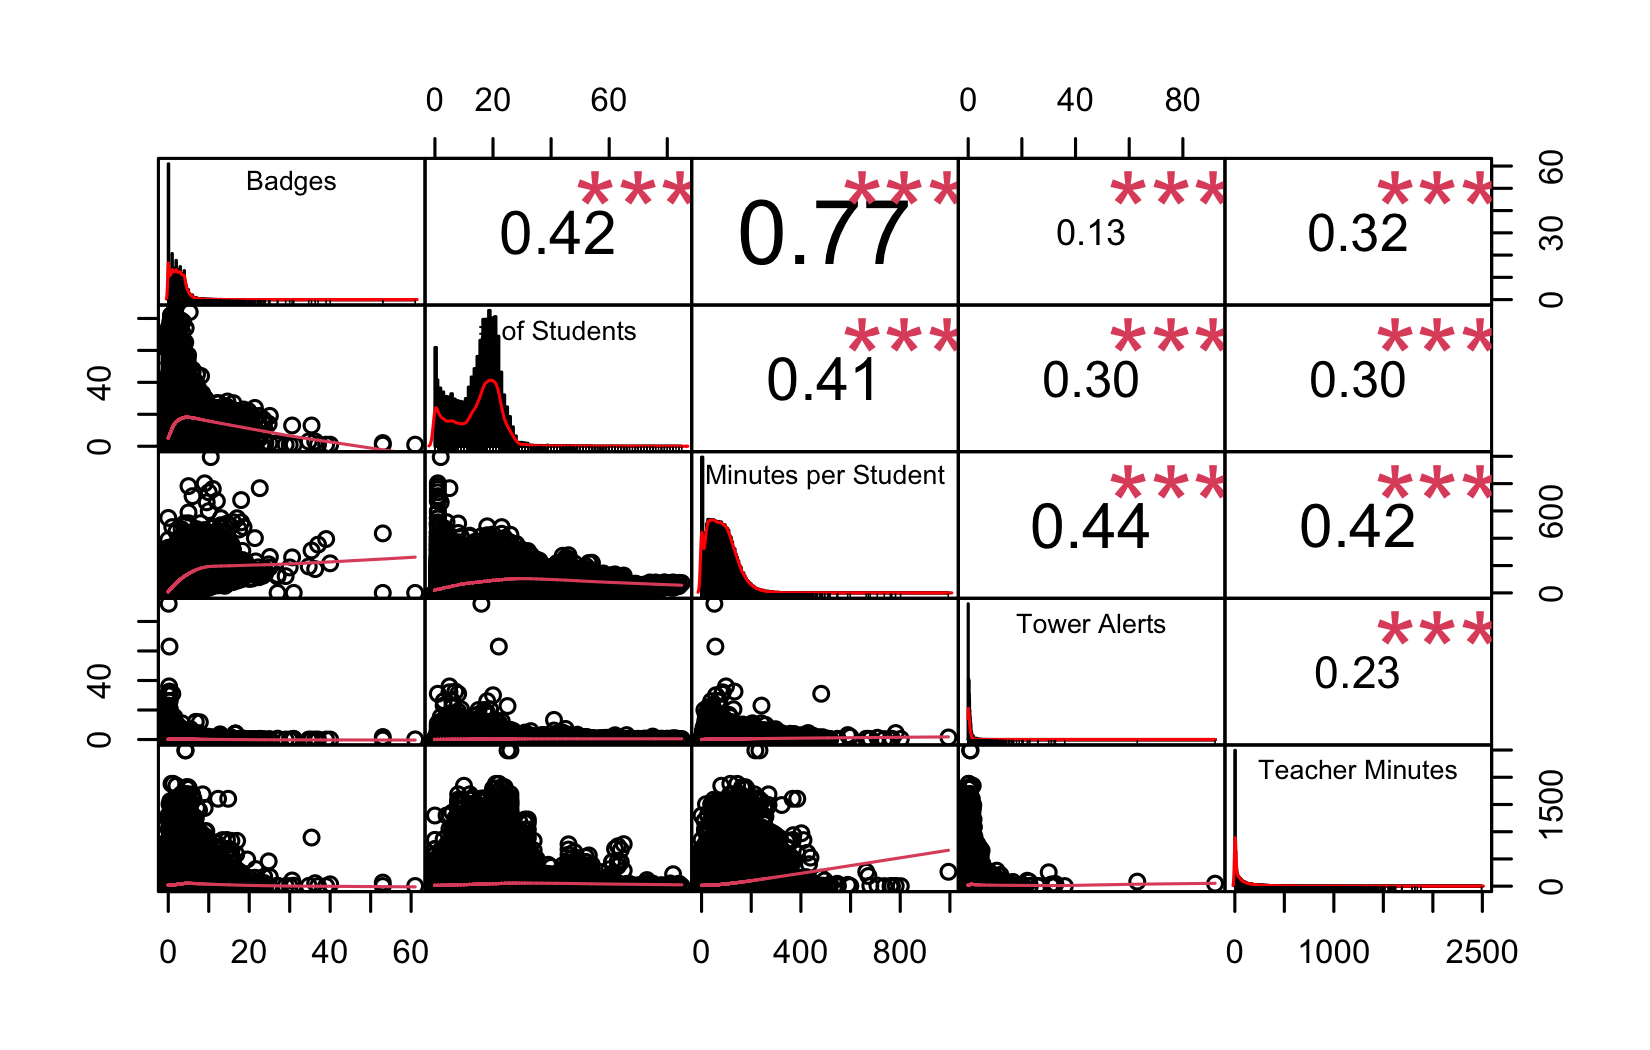
\includegraphics[keepaspectratio]{zearn_files/figure-pdf/fig-corr-1.png}}

}

\caption{\label{fig-corr}Correlation coefficients between variables
after stardardization}

\end{figure}%

\subsection{Supplemental Tables}\label{supplemental-tables}

\subsubsection{Teacher Variables}\label{teacher-variables}

\begin{longtable}[]{@{}
  >{\raggedright\arraybackslash}p{(\linewidth - 2\tabcolsep) * \real{0.2778}}
  >{\raggedright\arraybackslash}p{(\linewidth - 2\tabcolsep) * \real{0.7222}}@{}}
\caption{Catalog of Teacher Activities. This table presents teachers'
actions, including curriculum engagement, downloads of pedagogical
materials, and completion of various interactive components within the
Zearn educational platform.}\label{tbl-teacher-variables}\tabularnewline
\toprule\noalign{}
\begin{minipage}[b]{\linewidth}\raggedright
\textbf{Variable}
\end{minipage} & \begin{minipage}[b]{\linewidth}\raggedright
\textbf{Description}
\end{minipage} \\
\midrule\noalign{}
\endfirsthead
\toprule\noalign{}
\begin{minipage}[b]{\linewidth}\raggedright
\textbf{Variable}
\end{minipage} & \begin{minipage}[b]{\linewidth}\raggedright
\textbf{Description}
\end{minipage} \\
\midrule\noalign{}
\endhead
\bottomrule\noalign{}
\endlastfoot
PD Course Guide Download \citep{zearn2023, zearn2024c} & Detailed agenda
for Professional Development (PD) courses focusing on classroom
implementation, leadership, supporting diverse learners, using data to
inform teaching practices, and accelerating student learning. \\
PD Course Notes Download \citep{zearn2023, zearn2024c} & Professional
development session notes offering insights into effectively using
Zearn's curriculum. \\
Curriculum Map Download \citep{zearn2024d} & Detailed outline of
learning objectives and content. Presents a sequence of interconnected
math concepts across grades, aligning with states' instructional
requirements. \\
Assessments Download \citep{zearn2024e} & Assessments to evaluate
student understanding of the material, including ongoing formative
assessments, digital daily checks, and paper-based unit assessments. \\
Assessments Answer Key Download \citep{zearn2024f} & Solutions for
assessments to aid in grading and feedback. Provides detailed rubrics
for mission-level assessments. \\
Elementary Schedule Download \citep{zearn2024g} & A recommended schedule
for elementary school-level Zearn curriculum activities to guide daily
and weekly instructional planning, ensuring comprehensive coverage of
curriculum content. \\
Grade Level Overview Download \citep{zearn2024h} & Provides a summary of
learning objectives, pacing guidance, key grade-level terminology, a
list of required materials, and details on the standards covered by each
lesson. \\
Kindergarten Schedule Download \citep{zearn2024i} & Recommended
schedules for Kindergarten, supporting structured instruction
planning. \\
Kindergarten Mission Download \citep{zearn2024j} & Details interactive
activities focused on kindergarten-level concepts and their learning
objectives. \\
Mission Overview Download \citep{zearn2024h} & Outlines a mission's
(i.e., learning module) flow of topics, lessons, and assessments;
highlights foundational concepts introduced earlier; lists recently
introduced terms and required materials for teacher-led instruction. \\
Optional Homework Download \citep{zearn2024k} & Assignments for
additional practice, enhancing student learning outside of class. \\
Optional Problem Sets Download \citep{zearn2024l} & Exercises for extra
practice, tailored to reinforce lesson concepts. \\
Small Group Lesson Download \citep{zearn2024m} & Lessons designed for
small-group engagement. \\
Student Notes and Exit Tickets Download {[}\citep{zearn2024n};
@zearn2024o{]} & Student notes supplement digital lessons with
paper-and-pencil activities. Exit tickets are lesson-level assessments
for teachers to monitor daily learning. \\
Teaching and Learning Approach Download \citep{zearn2024p} & Resources
outlining Zearn's pedagogical methods. \\
Whole Group Fluency Download \citep{zearn2024q} & Lesson-aligned
practice activities to build math fluency through whole-class
engagement. \\
Whole Group Word Problems Download \citep{zearn2024m} & Word
problem-solving activities intended for collaborative, whole-class
engagement. \\
Fluency Completed \citep{zearn2024q} & Indicates teacher completed a
fluency activity, typically given to students before their daily digital
lessons. \\
Guided Practice Completed \citep{zearn2024r} & Indicates teacher
completed a guided practice segment, where students learn new concepts.
These include videos with on-screen teachers, interactive activities,
and paper-and-pencil Student Notes. \\
Kindergarten Activity Completed \citep{zearn2024s} & Indicates teacher
completed an activity within the Kindergarten curriculum. \\
Number Gym Activity Completed \citep{zearn2024t} & Indicates teacher
completed a Number Gym, an individually adaptive activity that builds
number sense, reinforces previously learned skills, and addresses areas
of unfinished learning. \\
Tower Completed \citep{zearn2024b} & Indicates teacher completed a Tower
of Power, an activity that requires full mastery of lesson objectives
and that students must complete independently. \\
Tower Struggled \citep{zearn2024u} & Indicates teacher committed a
mistake when engaging with the Tower of Power activity in a student
role, triggering a ``boost'' (scaffolding remediation). \\
Tower Stage Failed \citep{zearn2024b} & Indicates teacher received three
consecutive ``boosts'' due to repeated errors when engaging with the
Tower of Power in a student role. \\
\end{longtable}

\newpage{}

\begin{table}

\caption{\label{tbl-heterogeneity-reg}Relationship between Q-learning
Model Parameters and Classroom Characteristics. The table presents the
results of five regression models examining how reinforcement learning
(RL) parameters predict income and poverty levels, number of students,
number of classes per teacher, and whether the school had a paid Zearn
subscription. Coefficients and standard errors (in parentheses) are
provided for each parameter. Income and Poverty are treated as ordinal
variables, while Total Students and Number of Classes are count
variables. Paid Account is a binary variable. All RL parameters are
standardized (z-scored) before analysis.}

\centering{

\begin{verbatim}

% Table created by stargazer v.5.2.3 by Marek Hlavac, Social Policy Institute. E-mail: marek.hlavac at gmail.com
% Date and time: Fri, May 02, 2025 - 20:06:22
% Requires LaTeX packages: dcolumn 
\begin{table}[!htbp] \centering 
  \caption{Relationship between RL Parameters and Classroom Characteristics} 
  \label{} 
\begin{tabular}{@{\extracolsep{5pt}}lD{.}{.}{-3} D{.}{.}{-3} D{.}{.}{-3} D{.}{.}{-3} D{.}{.}{-3} } 
\\[-1.8ex]\hline 
\hline \\[-1.8ex] 
 & \multicolumn{5}{c}{\textit{Dependent variable:}} \\ 
\cline{2-6} 
\\[-1.8ex] & \multicolumn{1}{c}{Income} & \multicolumn{1}{c}{Poverty} & \multicolumn{1}{c}{Total Students} & \multicolumn{1}{c}{No. of Classes} & \multicolumn{1}{c}{Paid Account} \\ 
\\[-1.8ex] & \multicolumn{1}{c}{\textit{ordered}} & \multicolumn{1}{c}{\textit{ordered}} & \multicolumn{1}{c}{\textit{Poisson}} & \multicolumn{1}{c}{\textit{Poisson}} & \multicolumn{1}{c}{\textit{logistic}} \\ 
 & \multicolumn{1}{c}{\textit{logistic}} & \multicolumn{1}{c}{\textit{logistic}} & \multicolumn{1}{c}{\textit{}} & \multicolumn{1}{c}{\textit{}} & \multicolumn{1}{c}{\textit{}} \\ 
\\[-1.8ex] & \multicolumn{1}{c}{(1)} & \multicolumn{1}{c}{(2)} & \multicolumn{1}{c}{(3)} & \multicolumn{1}{c}{(4)} & \multicolumn{1}{c}{(5)}\\ 
\hline \\[-1.8ex] 
 Learning Rate ($\alpha$) & -0.113^{*} & 0.007 & 0.004 & 0.019 & 0.198^{*} \\ 
  & (0.049) & (0.055) & (0.006) & (0.019) & (0.084) \\ 
  & & & & & \\ 
 Discount Factor ($\gamma$) & -0.045 & 0.077 & -0.007 & -0.036 & 0.077 \\ 
  & (0.052) & (0.058) & (0.006) & (0.020) & (0.093) \\ 
  & & & & & \\ 
 Inverse Temperature ($\tau$) & 0.028 & -0.040 & 0.008 & -0.023 & 0.044 \\ 
  & (0.046) & (0.049) & (0.005) & (0.019) & (0.070) \\ 
  & & & & & \\ 
 Initial Q-value & 0.219^{***} & 0.025 & -0.002 & -0.009 & -0.237^{*} \\ 
  & (0.050) & (0.056) & (0.006) & (0.019) & (0.093) \\ 
  & & & & & \\ 
 Cost & -0.325^{***} & 0.191^{***} & -0.014^{*} & -0.057^{**} & 0.689^{***} \\ 
  & (0.049) & (0.057) & (0.006) & (0.019) & (0.119) \\ 
  & & & & & \\ 
 Constant &  &  & 3.027^{***} & 0.756^{***} & 2.145^{***} \\ 
  &  &  & (0.005) & (0.016) & (0.086) \\ 
  & & & & & \\ 
\hline \\[-1.8ex] 
Observations & \multicolumn{1}{c}{1,737} & \multicolumn{1}{c}{1,668} & \multicolumn{1}{c}{1,782} & \multicolumn{1}{c}{1,782} & \multicolumn{1}{c}{1,782} \\ 
Log Likelihood &  &  & \multicolumn{1}{c}{-5,728.098} & \multicolumn{1}{c}{-2,671.068} & \multicolumn{1}{c}{-628.413} \\ 
Akaike Inf. Crit. &  &  & \multicolumn{1}{c}{11,468.200} & \multicolumn{1}{c}{5,354.136} & \multicolumn{1}{c}{1,268.826} \\ 
\hline 
\hline \\[-1.8ex] 
\textit{Note:}  & \multicolumn{5}{r}{$^{*}$p$<$0.05; $^{**}$p$<$0.01; $^{***}$p$<$0.001} \\ 
\end{tabular} 
\end{table} 
\end{verbatim}

}

\end{table}%

\begin{table}

\caption{\label{tbl-optimality-2}Impact of Q-learning Model Parameters
on Average Weekly Tower Alerts per Tower Completion. Three linear
regression models examine the correlations between a teacher's
reinforcement learning (RL) parameters and student struggle, measured by
average weekly Tower Alerts. Model 1 includes only RL parameters. Model
2 adds controls for AIC, number of weeks, total students, and number of
classes. Model 3 further incorporates controls for grade level, poverty
level, charter school status, and whether the school has a paid Zearn
account. Coefficients and standard errors (in parentheses) are provided
for each parameter.}

\centering{

 \centering 
  \caption{} 
  \label{} 
\begin{tabular}{@{\extracolsep{5pt}}lD{.}{.}{-3} D{.}{.}{-3} D{.}{.}{-3} } 
\\[-1.8ex]\hline 
\hline \\[-1.8ex] 
 & \multicolumn{3}{c}{\textit{Dependent variable:}} \\ 
\cline{2-4} 
\\[-1.8ex] & \multicolumn{3}{c}{Tower Alerts} \\ 
\\[-1.8ex] & \multicolumn{1}{c}{(1)} & \multicolumn{1}{c}{(2)} & \multicolumn{1}{c}{(3)}\\ 
\hline \\[-1.8ex] 
 $\alpha$ & 0.059^{***} & 0.060^{***} & 0.054^{***} \\ 
  & (0.015) & (0.015) & (0.015) \\ 
  & & & \\ 
 $\gamma$ & 0.013 & 0.035^{*} & 0.042^{*} \\ 
  & (0.017) & (0.018) & (0.017) \\ 
  & & & \\ 
 $\tau$ & -0.031 & -0.098^{***} & -0.113^{***} \\ 
  & (0.017) & (0.028) & (0.027) \\ 
  & & & \\ 
 Cost & 0.028 & -0.007 & -0.016 \\ 
  & (0.017) & (0.022) & (0.021) \\ 
  & & & \\ 
 Starting Q-value & -0.006 & 0.030 & 0.049^{*} \\ 
  & (0.019) & (0.020) & (0.020) \\ 
  & & & \\ 
 No. of Weeks &  & 0.005^{*} & 0.005 \\ 
  &  & (0.003) & (0.003) \\ 
  & & & \\ 
 No. of Students &  & -0.006^{**} & -0.008^{***} \\ 
  &  & (0.002) & (0.002) \\ 
  & & & \\ 
 No. of Classes &  & 0.064^{***} & -0.012 \\ 
  &  & (0.013) & (0.016) \\ 
  & & & \\ 
 Charter School &  &  & -0.021 \\ 
  &  &  & (0.052) \\ 
  & & & \\ 
 Paid Zearn Account &  &  & 0.134^{***} \\ 
  &  &  & (0.038) \\ 
  & & & \\ 
 Constant & 0.934^{***} & 1.036^{***} & 0.211 \\ 
  & (0.013) & (0.142) & (0.205) \\ 
  & & & \\ 
\hline \\[-1.8ex] 
Control for AIC &  & Yes & Yes \\ 
Control for Grade Level &  &  & Yes \\ 
Control for Poverty Level &  &  & Yes \\ 
Observations & \multicolumn{1}{c}{1,782} & \multicolumn{1}{c}{1,782} & \multicolumn{1}{c}{1,668} \\ 
R$^{2}$ & \multicolumn{1}{c}{0.023} & \multicolumn{1}{c}{0.054} & \multicolumn{1}{c}{0.166} \\ 
Adjusted R$^{2}$ & \multicolumn{1}{c}{0.020} & \multicolumn{1}{c}{0.049} & \multicolumn{1}{c}{0.157} \\ 
Residual Std. Error & \multicolumn{1}{c}{0.535 (df = 1776)} & \multicolumn{1}{c}{0.527 (df = 1772)} & \multicolumn{1}{c}{0.497 (df = 1649)} \\ 
F Statistic & \multicolumn{1}{c}{8.198$^{***}$ (df = 5; 1776)} & \multicolumn{1}{c}{11.224$^{***}$ (df = 9; 1772)} & \multicolumn{1}{c}{18.223$^{***}$ (df = 18; 1649)} \\ 
\hline 
\hline \\[-1.8ex] 
\textit{Note:}  & \multicolumn{3}{r}{$^{*}$p$<$0.05; $^{**}$p$<$0.01; $^{***}$p$<$0.001} \\ 
\end{tabular} 

}

\end{table}%

\subsection{Supplemental Figures}\label{sec-supp-fig}

\begin{figure}

\centering{

\pandocbounded{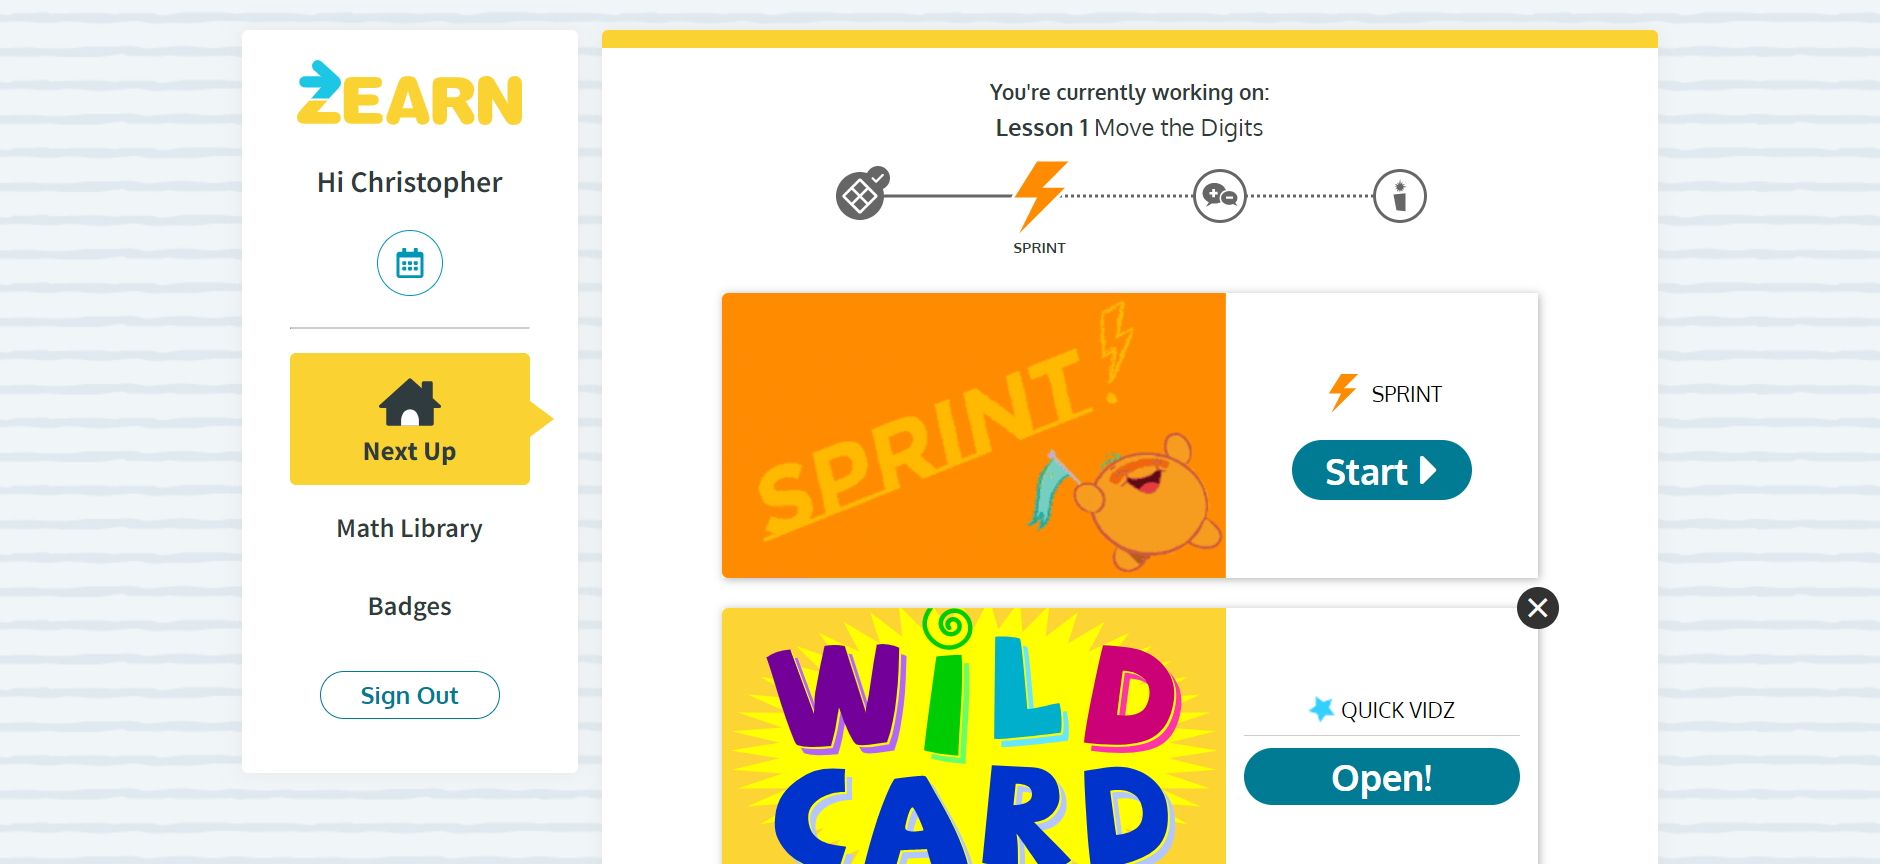
\includegraphics[keepaspectratio]{images/student-feed.PNG}}

}

\caption{\label{fig-st-portal}Zearn Student Portal}

\end{figure}%

\begin{figure}

\centering{

\pandocbounded{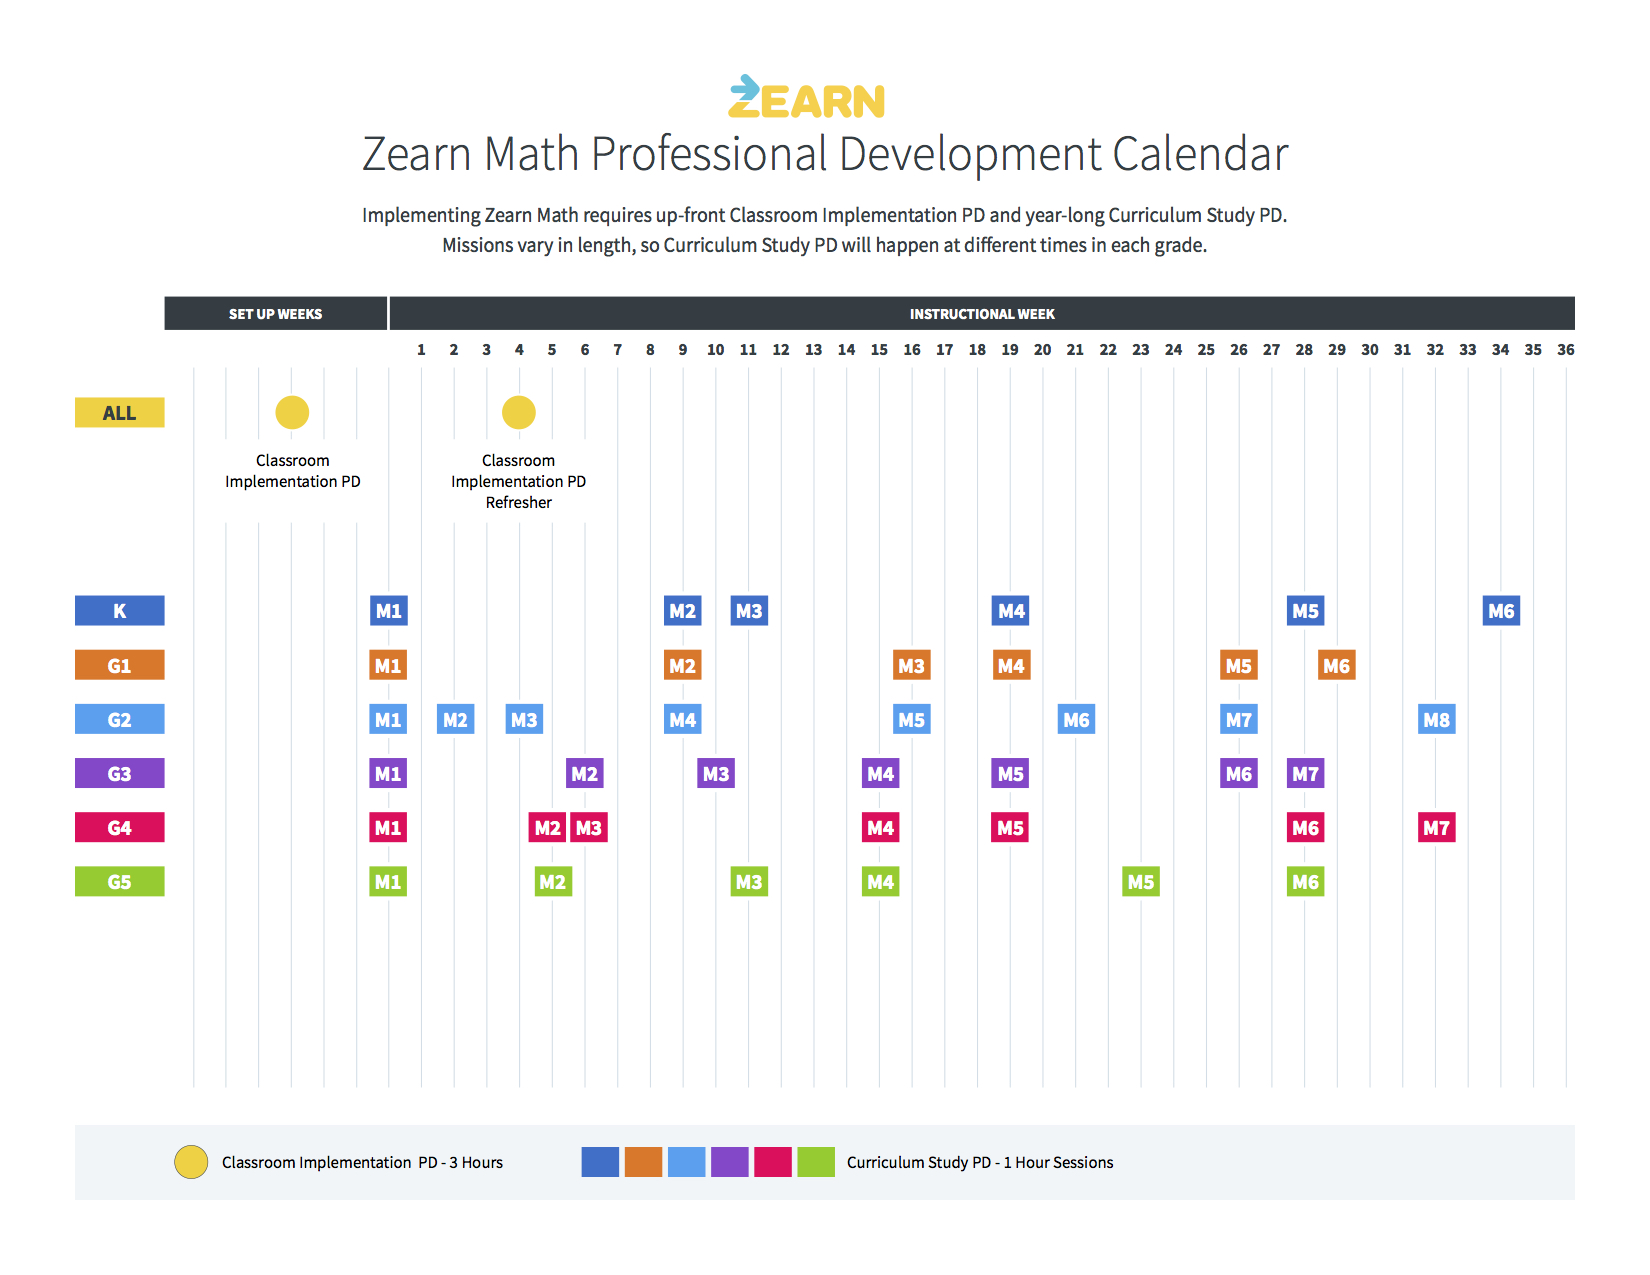
\includegraphics[keepaspectratio]{images/PD-calendar.jpg}}

}

\caption{\label{fig-prof-dev}Professional Development Calendar}

\end{figure}%

\newpage{}

\begin{figure}

\begin{minipage}{0.50\linewidth}

\centering{

\pandocbounded{\includegraphics[keepaspectratio]{zearn_files/figure-pdf/fig-income-dist-1.pdf}}

}

\subcaption{\label{fig-income-dist-1}School Poverty Distribution}

\end{minipage}%
%
\begin{minipage}{0.50\linewidth}

\centering{

\pandocbounded{\includegraphics[keepaspectratio]{zearn_files/figure-pdf/fig-income-dist-2.pdf}}

}

\subcaption{\label{fig-income-dist-2}Median Income Distribution}

\end{minipage}%

\caption{\label{fig-income-dist}Distributions of School Socioeconomic
Profiles. The first graph categorizes schools into three groups based on
the percentage of students eligible for free or reduced-price lunch
(FRPL): low-poverty (0-40\%), mid-poverty (40-75\%), and high-poverty
(over 75\%). The second graph presents the distribution of median
incomes for a school's associated region.}

\end{figure}%

\begin{figure}

\centering{

\pandocbounded{\includegraphics[keepaspectratio]{zearn_files/figure-pdf/fig-teachers-map-1.pdf}}

}

\caption{\label{fig-teachers-map}Geographic distribution of Zearn
teachers across parishes in Louisiana. The color gradient represents the
density of teachers, with darker hues indicating a higher concentration
of educators using Zearn in each parish. The map also labels the top
five cities where Zearn adoption is most prevalent.}

\end{figure}%

\begin{figure}

\centering{

\pandocbounded{\includegraphics[keepaspectratio]{zearn_files/figure-pdf/fig-logins-week-1.pdf}}

}

\caption{\label{fig-logins-week}Total number of student logins over the
2019-2020 school year. The chart depicts the connection between academic
schedules and platform engagement. Each bar represents a week, with
peaks corresponding to active school weeks and troughs aligning with
major holiday periods (e.g., Thanksgiving and Winter Break).}

\end{figure}%

\newpage{}

\begin{figure}

\begin{minipage}{\linewidth}

\centering{

\pandocbounded{\includegraphics[keepaspectratio]{zearn_files/figure-pdf/fig-nmf-pca-comparison-1.pdf}}

}

\subcaption{\label{fig-nmf-pca-comparison-1}Teacher Data}

\end{minipage}%
\newline
\begin{minipage}{\linewidth}

\centering{

\pandocbounded{\includegraphics[keepaspectratio]{zearn_files/figure-pdf/fig-nmf-pca-comparison-2.pdf}}

}

\subcaption{\label{fig-nmf-pca-comparison-2}Student Data}

\end{minipage}%

\caption{\label{fig-nmf-pca-comparison}Comparison of dimensionality
reduction techniques for teacher and student data. The figures compare
the performance of Principal Component Analysis (PCA) against
Nonnegative Matrix Factorization (NMF) in reducing the dimensionality of
teacher and student data. The NMF variants include the Frobenius norm
with two different initialization strategies: Nonnegative Double
Singular Value Decomposition (Frobenius NNDSVD) and NNDSVD with the
average of the input matrix X filled in place of zeros (Frobenius
NNDSVDA). The third NMF variant uses the Kullback-Leibler divergence as
the loss function. The left column assesses reconstruction quality using
R-squared, where values closer to 1 indicate that the components can
better recover the original data. The right column evaluates the
interpretability of the low-dimensional representation using silhouette
scores. Higher silhouette scores relate to better-defined clusters,
values near 0 indicate overlapping clusters, and negative values
generally suggest that a sample has been assigned to the wrong cluster.}

\end{figure}%

\newpage{}

\begin{figure}

\centering{

\pandocbounded{\includegraphics[keepaspectratio]{zearn_files/figure-pdf/fig-aic-ecdf-1.pdf}}

}

\caption{\label{fig-aic-ecdf}Empirical Cumulative Distribution Function
(ECDF) of teacher-specific Akaike Information Criteria (AIC) for
different models. Lower AIC values indicate better model fit.}

\end{figure}%

\newpage{}

\begin{verbatim}
$`2`
\end{verbatim}

\begin{verbatim}

$`14`
\end{verbatim}

\begin{figure}

\centering{

\pandocbounded{\includegraphics[keepaspectratio]{zearn_files/figure-pdf/fig-action-percentages-1.pdf}}

}

\caption{\label{fig-action-percentages-1}Observed teacher behavior and
model predictions over the academic year. The graph shows the percentage
of times teachers chose to engage in Pedagogical Content activities. The
x-axis represents biweekly periods throughout the school year. The black
dashed line represents observed teacher behavior, while colored lines
represent predictions from different models. Shaded areas represent the
95\% confidence intervals for each model's predictions.}

\end{figure}%

\begin{figure}

\centering{

\pandocbounded{\includegraphics[keepaspectratio]{zearn_files/figure-pdf/fig-action-percentages-2.pdf}}

}

\caption{\label{fig-action-percentages-2}Observed teacher behavior and
model predictions over the academic year. The graph shows the percentage
of times teachers chose to engage in Pedagogical Content activities. The
x-axis represents biweekly periods throughout the school year. The black
dashed line represents observed teacher behavior, while colored lines
represent predictions from different models. Shaded areas represent the
95\% confidence intervals for each model's predictions.}

\end{figure}%

\begin{verbatim}
$`2`
\end{verbatim}

\begin{verbatim}

$`14`
\end{verbatim}

\begin{figure}

\centering{

\pandocbounded{\includegraphics[keepaspectratio]{zearn_files/figure-pdf/fig-action-percentages-balanced-1.pdf}}

}

\caption{\label{fig-action-percentages-balanced-1}Observed teacher
behavior and model predictions over the academic year. The graph shows
the percentage of times teachers chose to engage in Pedagogical Content
activities. The x-axis represents biweekly periods throughout the school
year. The black dashed line represents observed teacher behavior, while
colored lines represent predictions from different models. Shaded areas
represent the 95\% confidence intervals for each model's predictions.}

\end{figure}%

\begin{figure}

\centering{

\pandocbounded{\includegraphics[keepaspectratio]{zearn_files/figure-pdf/fig-action-percentages-balanced-2.pdf}}

}

\caption{\label{fig-action-percentages-balanced-2}Observed teacher
behavior and model predictions over the academic year. The graph shows
the percentage of times teachers chose to engage in Pedagogical Content
activities. The x-axis represents biweekly periods throughout the school
year. The black dashed line represents observed teacher behavior, while
colored lines represent predictions from different models. Shaded areas
represent the 95\% confidence intervals for each model's predictions.}

\end{figure}%

\newpage{}

\begin{figure}

\centering{

\pandocbounded{\includegraphics[keepaspectratio]{zearn_files/figure-pdf/fig-corr-rl-params-1.pdf}}

}

\caption{\label{fig-corr-rl-params}Correlation matrix and distributions
of reinforcement learning parameters and model fit. The figure
illustrates the pairwise Spearman correlations between key reinforcement
learning parameters and model fit (AIC) derived from Q-learning model.
The diagonal shows the distribution of each parameter, with histograms
for discrete variables and density plots for continuous variables. The
lower triangle displays scatterplots of pairwise relationships, with
locally weighted scatterplot smoothing (LOWESS) lines in blue. The upper
triangle presents correlation coefficients, with asterisks indicating
statistical significance (\emph{p \textless{} 0.05, \textbf{p
\textless{} 0.01, }}p \textless{} 0.001).}

\end{figure}%





\end{document}
